\section{บทที่ 4 การลดรูปแผนภาพบล็อกและกราฟการไหลของสัญญาณ}

\noindent\textbf{ชื่อบทภาษาอังกฤษ:} Block Diagram Reduction and Signal Flow Graph\par
\noindent\textbf{รายวิชา:} ระบบควบคุม


\subsection{1. แนวคิดสำคัญของบท}

ระบบควบคุมในทางปฏิบัติมักประกอบด้วยระบบย่อยหลายส่วนที่เชื่อมต่อกัน เช่น ตัวควบคุม (controller) ตัวขับ (actuator) พลานต์ (plant) และเซนเซอร์ป้อนกลับ (feedback sensor) เมื่อสร้างแบบจำลองทางคณิตศาสตร์ของแต่ละส่วนได้ในรูป transfer function แล้ว ขั้นตอนถัดไปที่จำเป็นคือการนำ transfer function ย่อยเหล่านั้นมารวมกันเป็น transfer function เดียวของระบบทั้งหมด เพื่อนำไปวิเคราะห์เสถียรภาพ (stability) การตอบสนองชั่วครู่ (transient response) และการออกแบบตัวควบคุมในบทถัดไป

\textbf{Block Diagram} เป็นเครื่องมือมาตรฐานที่ใช้แสดงความสัมพันธ์เชิงฟังก์ชันระหว่างสัญญาณและระบบย่อยด้วยภาพ ทำให้เข้าใจโครงสร้างของระบบควบคุมได้ง่าย แต่เมื่อระบบมีหลายลูปป้อนกลับซ้อนกัน การลดรูปด้วยกฎพีชคณิตของแผนภาพบล็อกอาจทำได้ยากและเกิดข้อผิดพลาดสูง \textbf{Signal Flow Graph (SFG)} จึงถูกพัฒนาขึ้นเป็นอีกแนวทางหนึ่งที่ใช้กราฟทิศทางแทนความสัมพันธ์เชิงเส้น และอาศัย \textbf{Mason's Gain Formula} ในการคำนวณ transfer function โดยตรงจากโครงสร้างกราฟ โดยไม่ต้องลดรูปทีละขั้นตอน

บทนี้มุ่งให้ผู้เรียนสามารถลดรูปแผนภาพบล็อกด้วยกฎพีชคณิตพื้นฐาน อ่านและสร้าง Signal Flow Graph จากแผนภาพบล็อกหรือสมการของระบบ และประยุกต์ใช้ Mason's Gain Formula เพื่อหา transfer function ของระบบที่มีโครงสร้างซับซ้อนได้อย่างถูกต้องและเป็นระบบ พร้อมทั้งฝึกยืนยันผลด้วย MATLAB และ Simulink



\subsection{2. ความรู้พื้นฐานก่อนเรียน}

ผู้เรียนควรมีความรู้พื้นฐานต่อไปนี้ก่อนเข้าสู่บทที่ 4

\begin{itemize}
    \item \textbf{Laplace Transform} และการแปลงสมการเชิงอนุพันธ์เชิงเส้นจากโดเมนเวลาสู่โดเมน $s$
    \item ความหมายของ \textbf{Transfer Function}: $G(s) = \dfrac{\mathcal{L}\{\text{output}\}}{\mathcal{L}\{\text{input}\}}$ ภายใต้เงื่อนไขค่าเริ่มต้นเป็นศูนย์ (zero initial conditions)
    \item การสร้างแบบจำลองทางคณิตศาสตร์ของระบบทางกล ไฟฟ้า และระบบเชิงกล-ไฟฟ้า (ต่อเนื่องจากบทที่ 3)
    \item พีชคณิตพื้นฐาน การจัดรูปเศษส่วน และการแยกตัวประกอบพหุนาม
    \item แนวคิดพื้นฐานของระบบป้อนกลับ (feedback) และเครื่องหมายบวก/ลบที่จุดรวมสัญญาณ
    \item ความคุ้นเคยเบื้องต้นกับ MATLAB คำสั่งพื้นฐาน และการนิยามฟังก์ชันถ่ายโอนด้วยคำสั่ง \texttt{tf()}
\end{itemize}


\subsection{3. คำสำคัญประจำบท}

\textbf{ตารางที่ 1} คำสำคัญประจำบทที่ 4

\begin{table}[htbp]
    \centering
    \begin{tabularx}{\textwidth}{L{0.20\textwidth} L{0.24\textwidth} Y}
        \hline
        \textbf{คำศัพท์ภาษาไทย} & \textbf{English Term} & \textbf{ความหมายโดยย่อ} \\
        \hline
        แผนภาพบล็อก & Block Diagram & ภาพแสดงความสัมพันธ์เชิงฟังก์ชันระหว่างสัญญาณและระบบย่อยด้วยบล็อกและลูกศร \\
        บล็อก & Block & สัญลักษณ์แทนระบบย่อยหนึ่งส่วน กำกับด้วย transfer function \\
        จุดรวมสัญญาณ & Summing Junction & จุดที่สัญญาณตั้งแต่สองสัญญาณขึ้นไปถูกบวกหรือลบกัน \\
        จุดแยกสัญญาณ & Takeoff Point (Pickoff Point) & จุดที่สัญญาณเดียวกันถูกแยกส่งไปยังหลายเส้นทาง \\
        การต่อแบบอนุกรม & Series (Cascade) Connection & การต่อบล็อกเรียงต่อกันโดยเอาต์พุตของบล็อกหนึ่งเป็นอินพุตของบล็อกถัดไป \\
        การต่อแบบขนาน & Parallel Connection & การต่อบล็อกที่รับอินพุตเดียวกันแล้วนำเอาต์พุตมารวมกันที่จุดรวมสัญญาณ \\
        การป้อนกลับ & Feedback & การนำสัญญาณเอาต์พุตย้อนกลับมาเปรียบเทียบกับสัญญาณอินพุต \\
        ฟังก์ชันถ่ายโอนวงรอบปิด & Closed-Loop Transfer Function & transfer function ของระบบทั้งหมดหลังรวมลูปป้อนกลับแล้ว \\
        กราฟการไหลของสัญญาณ & Signal Flow Graph (SFG) & กราฟทิศทางที่แสดงความสัมพันธ์เชิงเส้นระหว่างตัวแปรด้วยโหนดและกิ่ง \\
        โหนด & Node & จุดในกราฟที่แทนตัวแปรหรือสัญญาณหนึ่งตัว \\
        กิ่ง & Branch & เส้นเชื่อมมีทิศทางระหว่างสองโหนด กำกับด้วยอัตราขยาย (gain) \\
        เส้นทาง & Path & ลำดับของกิ่งที่เชื่อมต่อกันตามทิศทางโดยไม่ผ่านโหนดซ้ำ \\
        เส้นทางหน้า & Forward Path & เส้นทางจากโหนดอินพุตไปยังโหนดเอาต์พุตโดยไม่ผ่านโหนดใดซ้ำ \\
        ลูป & Loop & เส้นทางปิดที่เริ่มต้นและสิ้นสุดที่โหนดเดียวกันโดยไม่ผ่านโหนดอื่นซ้ำ \\
        อัตราขยายลูป & Loop Gain & ผลคูณของอัตราขยายกิ่งทั้งหมดที่ประกอบเป็นลูปนั้น \\
        ลูปไม่สัมผัสกัน & Non-touching Loop & ลูปตั้งแต่สองลูปขึ้นไปที่ไม่มีโหนดร่วมกัน \\
        สูตรอัตราขยายเมสัน & Mason's Gain Formula & สูตรคำนวณ transfer function โดยตรงจากโครงสร้างของ Signal Flow Graph \\
        ดีเทอร์มิแนนต์ของกราฟ & Graph Determinant ($\Delta$) & ค่าที่คำนวณจากลูปทั้งหมดในกราฟ ใช้เป็นตัวหารในสูตรเมสัน \\
        โคแฟกเตอร์ของเส้นทาง & Path Cofactor ($\Delta_k$) & ค่า $\Delta$ ของส่วนกราฟที่ไม่สัมผัสกับเส้นทางหน้าที่ $k$ \\
        \hline
    \end{tabularx}
\end{table}


\subsection{4. ผลลัพธ์การเรียนรู้ประจำบท}

เมื่อเรียนจบบทนี้ นักศึกษาสามารถ

\begin{itemize}
    \item \textbf{CLO1:} อธิบายความหมายและองค์ประกอบของ Block Diagram ในระบบควบคุม รวมถึงความหมายของ Node, Branch, Path, Loop และ Non-touching Loop ใน Signal Flow Graph
    \item \textbf{CLO2:} จำแนกและอธิบายกฎการลดรูปแผนภาพบล็อกแต่ละแบบ ได้แก่ การต่อแบบอนุกรม แบบขนาน การป้อนกลับ การเลื่อนจุดรวมสัญญาณ และการเลื่อนจุดแยกสัญญาณ
    \item \textbf{CLO3:} คำนวณ transfer function ของระบบจากแผนภาพบล็อกโดยใช้กฎการลดรูปได้อย่างถูกต้อง
    \item \textbf{CLO4:} สร้าง Signal Flow Graph จากแผนภาพบล็อกหรือสมการของระบบ และคำนวณ transfer function ด้วย Mason's Gain Formula ได้อย่างถูกต้องเป็นระบบ
    \item \textbf{CLO5:} เปรียบเทียบข้อดีและข้อจำกัดของการลดรูปแผนภาพบล็อกกับการใช้ Signal Flow Graph และเลือกวิธีที่เหมาะสมกับลักษณะของระบบ
    \item \textbf{CLO6:} ยืนยันผลการคำนวณ transfer function ด้วยคำสั่ง MATLAB (\texttt{series}, \texttt{parallel}, \texttt{feedback}) และแบบจำลอง Simulink
\end{itemize}

\textbf{ตารางที่ 2} ตารางแสดงความสอดคล้องของผลลัพธ์การเรียนรู้ประจำบท (Curriculum Mapping)

\begin{table}[htbp]
    \centering
    \small
    \begin{tabularx}{\textwidth}{L{0.09\textwidth} L{0.16\textwidth} Y Y Y}
        \hline
        \textbf{ผลลัพธ์การเรียนรู้ประจำบท} & \textbf{เนื้อหาที่เกี่ยวข้อง} & \textbf{กิจกรรมการเรียนรู้} & \textbf{วิธีประเมิน} & \textbf{หลักฐานการเรียนรู้} \\
        \hline
        CLO1 & หัวข้อ 7.1–7.2, 7.5 & บรรยายพร้อมภาพประกอบ, คำถามกระตุ้นความคิดในชั้นเรียน & คำถามทบทวนข้อ 1–3, ทดสอบย่อย & คำตอบคำถามทบทวน, สมุดบันทึก \\
        CLO2 & หัวข้อ 7.3 & บรรยาย, วิเคราะห์ตัวอย่างที่ 1–3, กิจกรรมปฏิบัติการที่ 1 & แบบฝึกหัดระดับพื้นฐาน, สังเกตขณะฝึกลดรูปด้วยมือ & ใบงานกิจกรรมปฏิบัติการที่ 1 \\
        CLO3 & หัวข้อ 7.3–7.4, ตัวอย่างที่ 1–3 & ฝึกคำนวณตามขั้นตอน, กิจกรรมปฏิบัติการที่ 1 & แบบฝึกหัดระดับวิเคราะห์ข้อ 1–5 & ใบงาน, แบบฝึกหัดที่ส่ง \\
        CLO4 & หัวข้อ 7.5–7.6, ตัวอย่างที่ 4 & บรรยาย, ฝึกสร้างตารางคำนวณ Mason's Gain Formula, กิจกรรมปฏิบัติการที่ 4 & แบบฝึกหัดระดับวิเคราะห์และประยุกต์ & ตาราง $P_k$, Loop gain, $\Delta$, $\Delta_k$ ที่นักศึกษาจัดทำ \\
        CLO5 & หัวข้อ 7.7 & อภิปรายกลุ่มย่อย, เปรียบเทียบผลจากสองวิธี & คำถามทบทวนข้อ 8–9, แบบฝึกหัดระดับประยุกต์ & บันทึกการอภิปราย, คำตอบข้อเปรียบเทียบ \\
        CLO6 & หัวข้อ 7.8, กิจกรรมปฏิบัติการที่ 2–3 & ปฏิบัติการ MATLAB และ Simulink & ตรวจผลลัพธ์จากซอฟต์แวร์เทียบกับการคำนวณด้วยมือ & ไฟล์สคริปต์ MATLAB, ผลจำลอง Simulink \\
        \hline
    \end{tabularx}
\end{table}


\subsection{5. แผนผังเนื้อหาของบท}

ลำดับเนื้อหาของบทนี้จัดเรียงจากพื้นฐานไปสู่การประยุกต์ใช้ ดังนี้

\begin{enumerate}
    \item ความหมายและองค์ประกอบของ Block Diagram
    \item กฎการลดรูปแผนภาพบล็อก (อนุกรม $\rightarrow$ ขนาน $\rightarrow$ ป้อนกลับ $\rightarrow$ เลื่อนจุดรวมสัญญาณ/จุดแยกสัญญาณ)
    \item ขั้นตอนการลดรูปแผนภาพบล็อกที่มีหลายลูปซ้อนกัน
    \item Signal Flow Graph: Node, Branch, Path, Loop, Non-touching Loop
    \item Mason's Gain Formula และขั้นตอนการคำนวณ
    \item การเปรียบเทียบสองวิธี และการใช้ MATLAB/Simulink ยืนยันผล
    \item การประยุกต์ใช้ในงานจริง กิจกรรมปฏิบัติการ และแบบฝึกหัด
\end{enumerate}


\subsection{6. บทนำ}

ในบทที่ 3 ผู้เรียนได้ฝึกสร้างแบบจำลองทางคณิตศาสตร์ของระบบทางกล ไฟฟ้า และเชิงกล-ไฟฟ้าในรูป transfer function ของระบบย่อยแต่ละส่วน แต่ระบบควบคุมจริงแทบไม่เคยประกอบด้วยระบบย่อยเพียงส่วนเดียว ตัวอย่างเช่น ระบบควบคุมความเร็วมอเตอร์ประกอบด้วยตัวควบคุม (controller) วงจรขับกำลัง (driver) มอเตอร์ (plant) และเซนเซอร์วัดความเร็วที่ป้อนสัญญาณกลับมาเปรียบเทียบกับค่าที่ต้องการ ระบบกันสะเทือนของยานยนต์ ระบบควบคุมอุณหภูมิ หรือแม้แต่ระบบควบคุมท่าทางของโดรน ล้วนมีโครงสร้างเป็นบล็อกหลายส่วนเชื่อมต่อกันเป็นวงรอบป้อนกลับซ้อนกันหลายชั้น

วิศวกรระบบควบคุมจำเป็นต้องหา transfer function รวมของทั้งระบบ (เช่น อัตราส่วนระหว่างเอาต์พุตกับอินพุตอ้างอิง) เพื่อนำไปวิเคราะห์เสถียรภาพและออกแบบตัวควบคุมในบทถัดไป การหา transfer function รวมนี้ทำได้สองแนวทางหลัก คือ การใช้ \textbf{กฎการลดรูปแผนภาพบล็อก} ซึ่งใช้พีชคณิตของบล็อกทีละขั้นตอนจนเหลือบล็อกเดียว และการใช้ \textbf{Signal Flow Graph ร่วมกับ Mason's Gain Formula} ซึ่งคำนวณ transfer function ได้โดยตรงจากโครงสร้างกราฟโดยไม่ต้องลดรูปทีละขั้น ทั้งสองวิธีให้ผลลัพธ์เดียวกันเสมอ แต่มีความเหมาะสมต่างกันตามความซับซ้อนของระบบ ซึ่งเป็นประเด็นที่บทนี้จะอธิบายอย่างละเอียด


\subsection{7. เนื้อหาหลัก}

\subsubsection{7.1 ความหมายของ Block Diagram ในระบบควบคุม}

\textbf{Block Diagram} คือแผนภาพที่แสดงความสัมพันธ์เชิงฟังก์ชันระหว่างสัญญาณต่าง ๆ ในระบบด้วยบล็อกสี่เหลี่ยมและลูกศรแสดงทิศทางการไหลของสัญญาณ แต่ละบล็อกกำกับด้วย transfer function ของระบบย่อยนั้น โดยมีข้อสมมติสำคัญคือ \textbf{สัญญาณไหลไปในทิศทางเดียว} (unidirectional signal flow) และ \textbf{บล็อกที่ต่อกันไม่มีผลโหลด (loading effect) ต่อกัน} กล่าวคือ การต่อบล็อกหนึ่งเข้ากับอีกบล็อกหนึ่งจะไม่เปลี่ยนแปลงค่า transfer function เดิมของแต่ละบล็อก ซึ่งเป็นเงื่อนไขที่ทำให้สามารถใช้กฎพีชคณิตในการรวมบล็อกได้โดยตรง

ข้อดีของ Block Diagram คือทำให้เห็นโครงสร้างของระบบและเส้นทางของสัญญาณได้อย่างชัดเจนด้วยภาพ เหมาะสำหรับสื่อสารแนวคิดการออกแบบระหว่างวิศวกร และเป็นพื้นฐานสำคัญก่อนนำไปวิเคราะห์เสถียรภาพและออกแบบตัวควบคุมในบทถัดไป

% [รูปที่ 1: องค์ประกอบพื้นฐานของ Block Diagram]
% ประเภทภาพ: Technical Illustration
% ตำแหน่งที่แนะนำ: ท้ายหัวข้อ 7.1
% วัตถุประสงค์การเรียนรู้: ให้ผู้เรียนจดจำสัญลักษณ์พื้นฐานสามชนิดที่ประกอบเป็น Block Diagram ได้แก่ บล็อก จุดรวมสัญญาณ และจุดแยกสัญญาณ
% คำอธิบายภาพ: แสดงบล็อกสี่เหลี่ยมหนึ่งบล็อกกำกับด้วย $G(s)$ มีลูกศรอินพุต $R(s)$ เข้าทางซ้ายและลูกศรเอาต์พุต $C(s)$ ออกทางขวา ถัดไปแสดงวงกลมจุดรวมสัญญาณที่มีลูกศรเข้าสองเส้นกำกับเครื่องหมาย + และ − และลูกศรออกหนึ่งเส้น สุดท้ายแสดงจุดแยกสัญญาณเป็นจุดทึบบนเส้นสัญญาณที่แตกลูกศรออกเป็นสองเส้นไปยังปลายทางต่างกัน
% องค์ประกอบที่ต้องมี: บล็อกสี่เหลี่ยม, วงกลมจุดรวมสัญญาณพร้อมเครื่องหมาย +/−, จุดแยกสัญญาณ, ลูกศรแสดงทิศทางสัญญาณ, สัญลักษณ์ $R(s)$, $C(s)$, $G(s)$
% ข้อความหรือป้ายกำกับ: $R(s)$, $C(s)$, $G(s)$, เครื่องหมาย +, −
% ภาษาของป้ายกำกับ: ไทยและอังกฤษ
% สัดส่วนภาพ: 16:9
% Image Generation Prompt: Clean technical diagram for a control systems textbook showing three basic block-diagram symbols side by side: (1) a labeled rectangular block G(s) with an input arrow R(s) and output arrow C(s); (2) a summing junction circle with two input arrows marked + and − and one output arrow; (3) a takeoff point shown as a solid dot on a signal line splitting into two arrows. Minimalist black-and-white engineering diagram style, white background, clear labels, no shading, no photorealism.
% Alt Text: ภาพแสดงสัญลักษณ์พื้นฐานสามชนิดของแผนภาพบล็อก ได้แก่ บล็อกแทน transfer function จุดรวมสัญญาณที่มีเครื่องหมายบวกลบ และจุดแยกสัญญาณ

\begin{figure}[htbp]
    \centering
    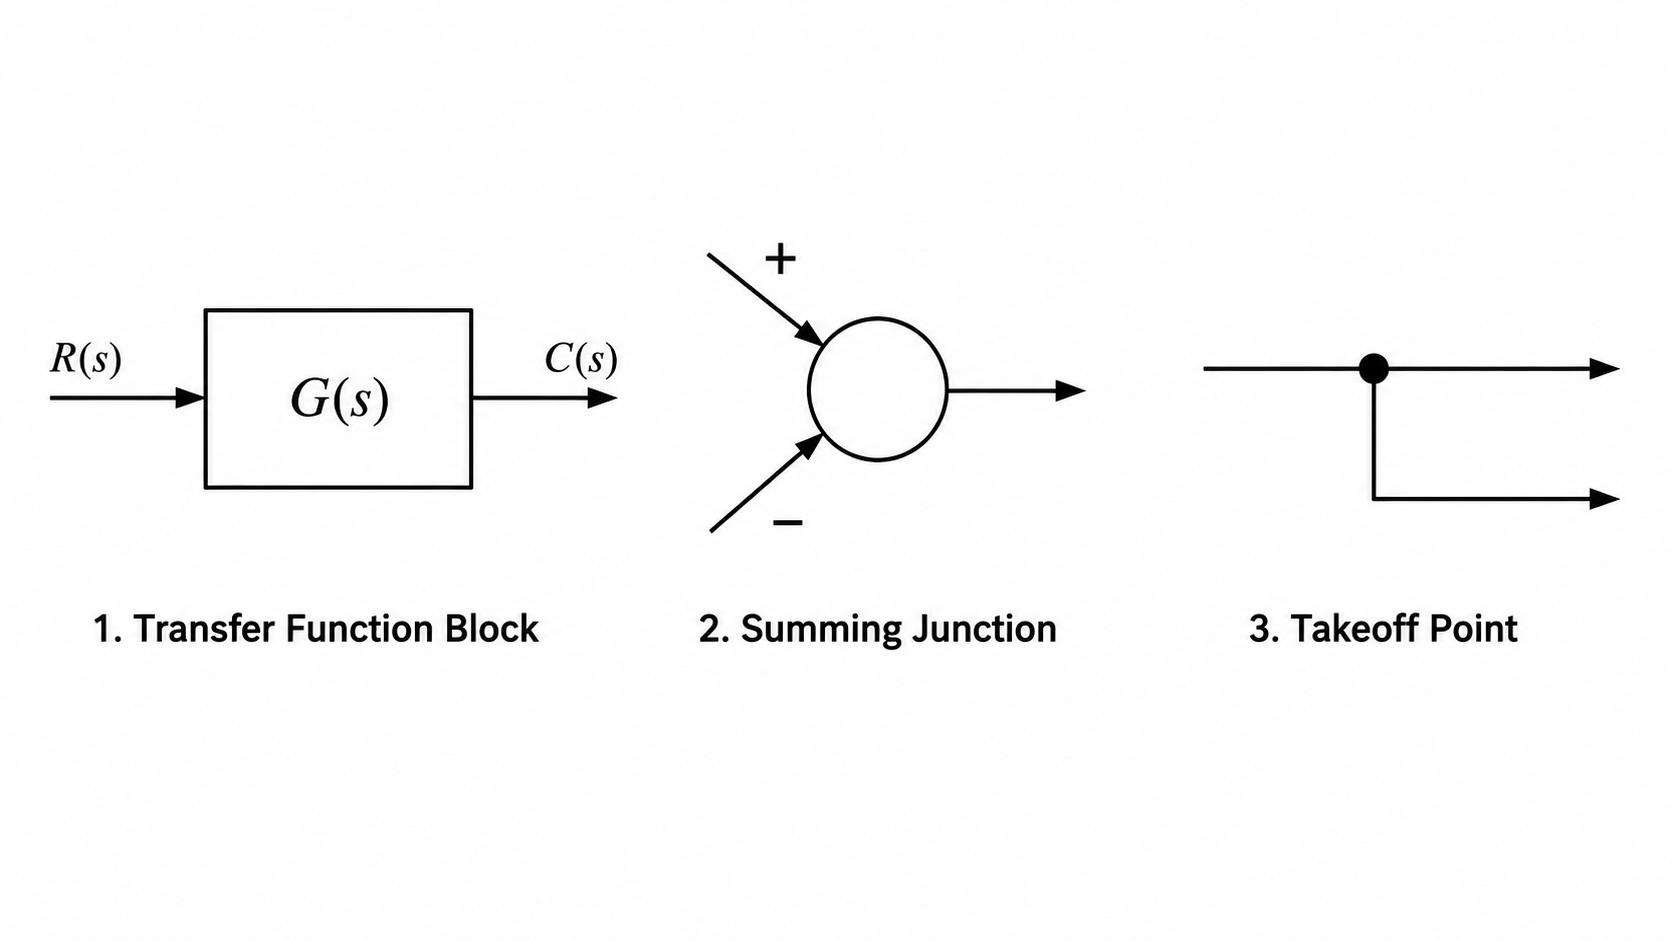
\includegraphics[width=0.8\textwidth]{images/chapter4/figure-01.png}
    \caption{องค์ประกอบพื้นฐานของ Block Diagram}
\end{figure}

\subsubsection{7.2 องค์ประกอบพื้นฐานของ Block Diagram}

Block Diagram ประกอบด้วยองค์ประกอบหลัก 4 ชนิด

\begin{enumerate}
    \item \textbf{บล็อก (Block):} แทนระบบย่อยหนึ่งส่วน กำกับด้วย transfer function เช่น $G(s)$ โดยเอาต์พุตของบล็อกคือผลคูณของอินพุตกับ transfer function ในโดเมน $s$ กล่าวคือ หากอินพุตคือ $X(s)$ เอาต์พุตคือ $Y(s) = G(s)X(s)$
    \item \textbf{เส้นสัญญาณ (Signal Line):} ลูกศรแสดงทิศทางการไหลของสัญญาณ สัญญาณไหลได้ทิศทางเดียวตามลูกศรเท่านั้น
    \item \textbf{จุดรวมสัญญาณ (Summing Junction):} วงกลมที่รวมสัญญาณตั้งแต่สองสัญญาณขึ้นไปด้วยการบวกหรือลบตามเครื่องหมายกำกับที่ทางเข้าแต่ละเส้น เช่น $E(s) = R(s) - B(s)$
    \item \textbf{จุดแยกสัญญาณ (Takeoff Point หรือ Pickoff Point):} จุดที่สัญญาณเดียวกันถูกส่งไปยังหลายเส้นทางพร้อมกันโดยไม่เปลี่ยนแปลงค่า
\end{enumerate}

\subsubsection{7.3 กฎการลดรูปแผนภาพบล็อก}

การลดรูปแผนภาพบล็อก (Block Diagram Reduction) คือกระบวนการรวมบล็อกที่เชื่อมต่อกันตามกฎพีชคณิตทีละขั้นตอน จนเหลือบล็อกเดียวที่แทน transfer function รวมของระบบ กฎพื้นฐานที่ใช้บ่อยที่สุดมี 3 กฎหลัก ได้แก่ การต่อแบบอนุกรม การต่อแบบขนาน และการป้อนกลับ ร่วมกับกฎเสริมอีก 2 กฎสำหรับจัดการตำแหน่งของจุดรวมสัญญาณและจุดแยกสัญญาณเมื่อกฎหลักไม่สามารถใช้ได้โดยตรง

\paragraph{7.3.1 การต่อแบบอนุกรม (Series/Cascade Connection)}

เมื่อบล็อกสองบล็อกต่อกันโดยเอาต์พุตของบล็อกแรกเป็นอินพุตของบล็อกถัดไปโดยตรง (ไม่มีจุดแยกสัญญาณหรือจุดรวมสัญญาณคั่นกลาง) เรียกว่าการต่อแบบอนุกรม transfer function รวมคือผลคูณของ transfer function แต่ละบล็อก

\[
G_{eq}(s) = G_1(s) \, G_2(s)
\]

% [รูปที่ 2: การต่อแบบอนุกรมและผลลัพธ์การลดรูป]
% ประเภทภาพ: Block Diagram
% ตำแหน่งที่แนะนำ: ท้ายหัวข้อ 7.3.1 ก่อนตัวอย่างที่ 1
% วัตถุประสงค์การเรียนรู้: แสดงการแปลงบล็อกสองบล็อกที่ต่ออนุกรมให้เป็นบล็อกเดียว
% คำอธิบายภาพ: แถวบนแสดง $R(s)$ เข้าบล็อก $G_1(s)$ ต่อด้วยบล็อก $G_2(s)$ แล้วออกเป็น $C(s)$ แถวล่างแสดงบล็อกเดียว $G_1(s)G_2(s)$ ที่รับ $R(s)$ และให้ผลลัพธ์ $C(s)$ เท่ากัน พร้อมลูกศร "เทียบเท่ากับ" คั่นกลางสองแถว
% องค์ประกอบที่ต้องมี: บล็อกสี่เหลี่ยมสองบล็อกในแถวบน บล็อกเดียวในแถวล่าง ลูกศรสัญญาณ สัญลักษณ์ "≡" หรือ "เทียบเท่ากับ" คั่นกลาง
% ข้อความหรือป้ายกำกับ: $R(s)$, $C(s)$, $G_1(s)$, $G_2(s)$, $G_1(s)G_2(s)$
% ภาษาของป้ายกำกับ: ไทยและอังกฤษ
% สัดส่วนภาพ: 16:9
% Image Generation Prompt: Control systems block diagram showing two rectangular blocks G1(s) and G2(s) connected in series with an input arrow R(s) and output arrow C(s) in the top row; below, an equivalence arrow points to a single equivalent block labeled G1(s)G2(s) with the same input R(s) and output C(s). Clean minimalist engineering diagram, white background, black lines, clear labels.
% Alt Text: ภาพแสดงบล็อกสองบล็อกต่ออนุกรมกันและบล็อกสมมูลบล็อกเดียวที่มีค่าเท่ากับผลคูณของ transfer function ทั้งสอง

\begin{figure}[htbp]
    \centering
    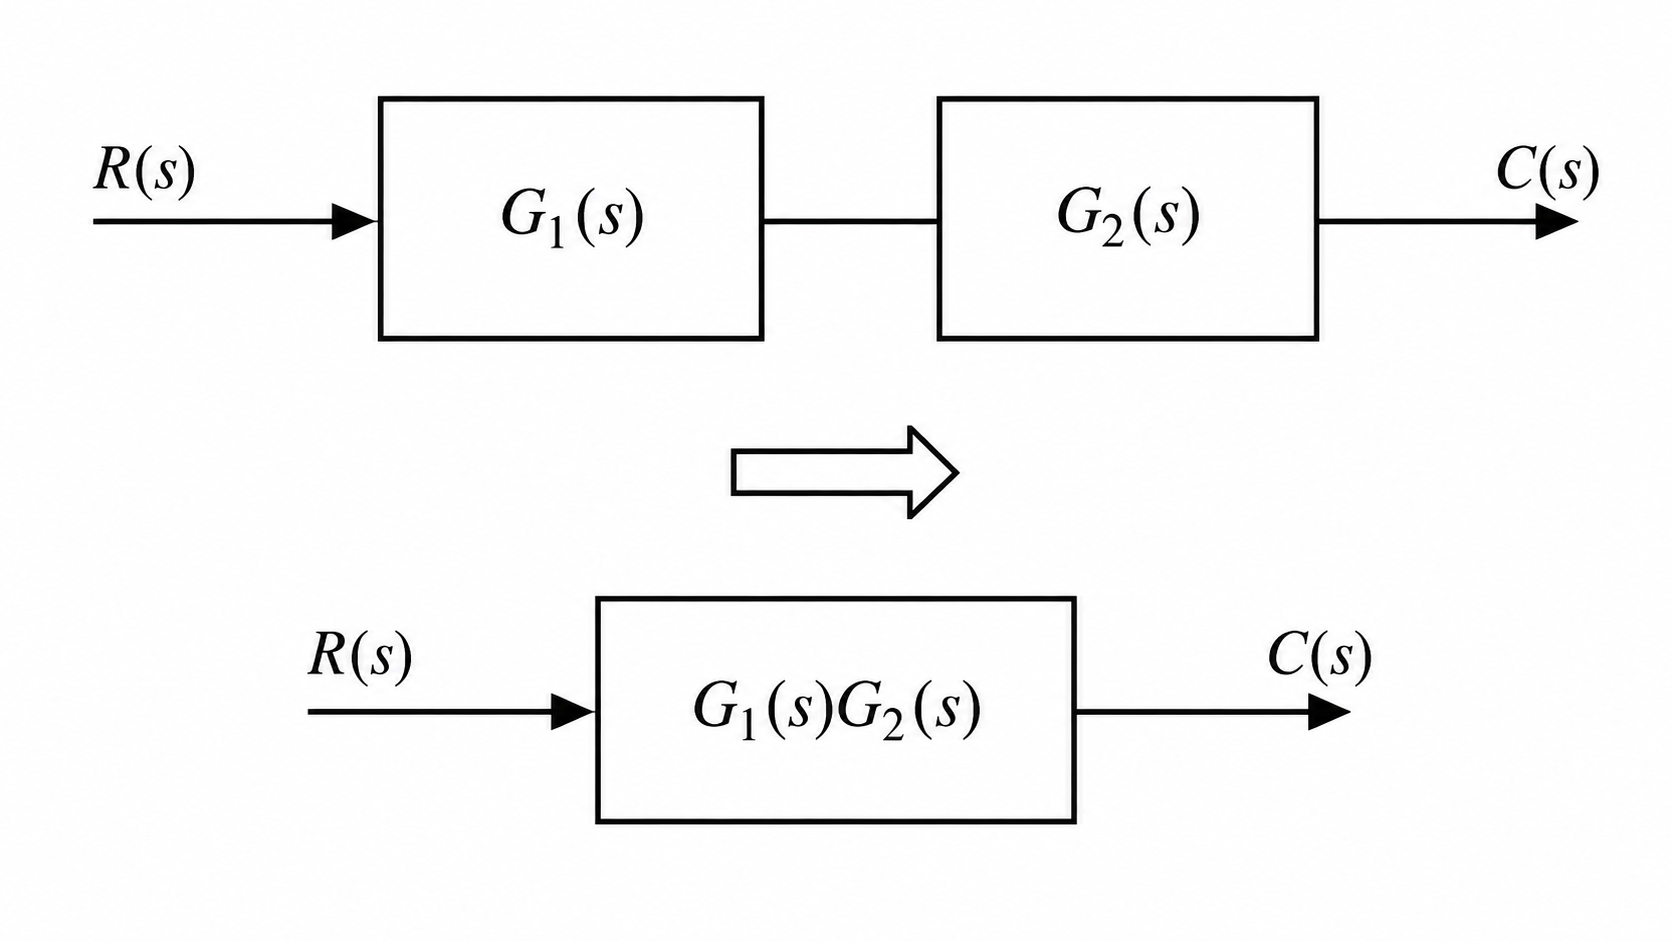
\includegraphics[width=0.8\textwidth]{images/chapter4/figure-02.png}
    \caption{การต่อแบบอนุกรมและผลลัพธ์การลดรูป}
\end{figure}

\textbf{ตัวอย่างที่ 1: การต่อแบบอนุกรม (Series)}

\textbf{โจทย์:} ระบบควบคุมประกอบด้วยตัวควบคุมและพลานต์ต่อกันแบบอนุกรม โดยตัวควบคุมมี transfer function $G_1(s) = \dfrac{1}{s+2}$ และพลานต์มี transfer function $G_2(s) = \dfrac{5}{s+4}$ จงหา transfer function รวม $C(s)/R(s)$

\textit{ขั้นตอนที่ 1 วิเคราะห์ระบบ:} บล็อกทั้งสองต่อกันโดยตรงแบบอนุกรม ไม่มีจุดรวมหรือจุดแยกสัญญาณคั่นกลาง จึงใช้กฎการต่อแบบอนุกรมได้ทันที

\textit{ขั้นตอนที่ 2 กำหนดตัวแปร:} $R(s)$ คืออินพุต $C(s)$ คือเอาต์พุต

\textit{ขั้นตอนที่ 3–4 เลือกกฎและสร้างสมการ:}

\[
G_{eq}(s) = G_1(s)\,G_2(s) = \frac{1}{s+2}\cdot\frac{5}{s+4}
\]

\textit{ขั้นตอนที่ 5–7 จัดรูปและคำนวณ:}

\[
G_{eq}(s) = \frac{5}{(s+2)(s+4)} = \frac{5}{s^2+6s+8}
\]

\textit{ขั้นตอนที่ 8 ตรวจสอบ:} ดีกรีของพหุนามส่วนเท่ากับผลรวมดีกรีของทั้งสองบล็อก (1+1 = 2) สอดคล้องกับสมบัติของระบบอันดับสอง ค่าคงตัวเวลา (time constant) ของแต่ละบล็อกเดิมยังปรากฏเป็นราก $s=-2$ และ $s=-4$ ของสมการส่วน ซึ่งสมเหตุสมผล

\textit{ขั้นตอนที่ 9 แปลความหมาย:} $C(s) = \dfrac{5}{s^2+6s+8}R(s)$ คือ transfer function รวมของตัวควบคุมและพลานต์ที่ต่ออนุกรมกัน พร้อมนำไปวิเคราะห์ในบทถัดไป

\paragraph{7.3.2 การต่อแบบขนาน (Parallel Connection)}

เมื่อบล็อกตั้งแต่สองบล็อกขึ้นไปรับสัญญาณอินพุตเดียวกัน แล้วนำเอาต์พุตของแต่ละบล็อกมารวมกันที่จุดรวมสัญญาณ เรียกว่าการต่อแบบขนาน transfer function รวมคือผลบวก (หรือผลต่าง ตามเครื่องหมายที่จุดรวมสัญญาณ) ของ transfer function แต่ละบล็อก

\[
G_{eq}(s) = G_1(s) \pm G_2(s)
\]

\textbf{ตัวอย่างที่ 2: การต่อแบบขนาน (Parallel)}

\textbf{โจทย์:} ระบบมีสองเส้นทางสัญญาณที่รับอินพุตเดียวกัน $R(s)$ แล้วนำเอาต์พุตมาบวกกันที่จุดรวมสัญญาณ โดย $G_1(s) = \dfrac{3}{s+1}$ และ $G_2(s) = \dfrac{2}{s+5}$ จงหา transfer function รวม $C(s)/R(s)$

\textit{ขั้นตอนที่ 1–2 วิเคราะห์และกำหนดตัวแปร:} ทั้งสองบล็อกรับ $R(s)$ เดียวกัน เอาต์พุตทั้งสองรวมกันเป็น $C(s) = G_1(s)R(s) + G_2(s)R(s)$

\textit{ขั้นตอนที่ 3–4 เลือกกฎและสร้างสมการ:}

\[
G_{eq}(s) = G_1(s) + G_2(s) = \frac{3}{s+1} + \frac{2}{s+5}
\]

\textit{ขั้นตอนที่ 5–7 จัดรูปเศษส่วนร่วมและคำนวณ:}

\[
G_{eq}(s) = \frac{3(s+5) + 2(s+1)}{(s+1)(s+5)} = \frac{3s+15+2s+2}{(s+1)(s+5)} = \frac{5s+17}{s^2+6s+5}
\]

\textit{ขั้นตอนที่ 8 ตรวจสอบ:} ดีกรีของพหุนามเศษต้องน้อยกว่าดีกรีของพหุนามส่วนหนึ่งลำดับ (proper transfer function) ในที่นี้เศษดีกรี 1 ส่วนดีกรี 2 ถูกต้องตามสมบัติของระบบเชิงเหตุ (causal system)

\textit{ขั้นตอนที่ 9 แปลความหมาย:} $G_{eq}(s) = \dfrac{5s+17}{s^2+6s+5}$ คือ transfer function รวมของสองเส้นทางที่ต่อขนานและบวกสัญญาณกันที่เอาต์พุต

\paragraph{7.3.3 การป้อนกลับ (Feedback)}

โครงสร้างป้อนกลับประกอบด้วยบล็อกเส้นทางไปข้างหน้า $G(s)$ (forward path) และบล็อกเส้นทางป้อนกลับ $H(s)$ (feedback path) โดยสัญญาณเอาต์พุตถูกป้อนกลับผ่าน $H(s)$ แล้วนำไปเปรียบเทียบกับสัญญาณอินพุตที่จุดรวมสัญญาณ หาก $H(s)=1$ เรียกว่า \textbf{ระบบป้อนกลับหนึ่งหน่วย (unity feedback)}

สำหรับ \textbf{ระบบป้อนกลับเชิงลบ (negative feedback)} สัญญาณผิดพลาด (error signal) คือ $E(s) = R(s) - H(s)C(s)$ และ $C(s) = G(s)E(s)$ เมื่อแทนค่าและจัดรูปจะได้

\[
\frac{C(s)}{R(s)} = \frac{G(s)}{1 + G(s)H(s)}
\]

ส่วน \textbf{ระบบป้อนกลับเชิงบวก (positive feedback)} ซึ่งสัญญาณป้อนกลับถูกบวกเข้ากับอินพุตแทนการลบ จะได้

\[
\frac{C(s)}{R(s)} = \frac{G(s)}{1 - G(s)H(s)}
\]

พจน์ $G(s)H(s)$ เรียกว่า \textbf{loop gain} ของระบบป้อนกลับ ซึ่งเป็นตัวแปรสำคัญที่ใช้วิเคราะห์เสถียรภาพในบทถัดไป

% [รูปที่ 3: โครงสร้างระบบป้อนกลับเชิงลบและเชิงบวก]
% ประเภทภาพ: Block Diagram
% ตำแหน่งที่แนะนำ: ท้ายหัวข้อ 7.3.3 ก่อนตัวอย่างที่ 3
% วัตถุประสงค์การเรียนรู้: ให้ผู้เรียนแยกแยะโครงสร้างและเครื่องหมายของระบบป้อนกลับเชิงลบกับเชิงบวก
% คำอธิบายภาพ: แสดงจุดรวมสัญญาณรับ $R(s)$ เข้าทางหนึ่งและสัญญาณป้อนกลับจาก $H(s)$ เข้าอีกทางหนึ่ง ผลลัพธ์ $E(s)$ เข้าบล็อก $G(s)$ แล้วออกเป็น $C(s)$ ซึ่งมีจุดแยกสัญญาณย้อนกลับเข้า $H(s)$ ก่อนกลับไปยังจุดรวมสัญญาณ ทำสองแบบคู่กันคือเครื่องหมาย − (เชิงลบ) และเครื่องหมาย + (เชิงบวก)
% องค์ประกอบที่ต้องมี: จุดรวมสัญญาณ บล็อก $G(s)$ บล็อก $H(s)$ จุดแยกสัญญาณ ลูกศรทิศทาง เครื่องหมาย +/−
% ข้อความหรือป้ายกำกับ: $R(s)$, $E(s)$, $C(s)$, $G(s)$, $H(s)$, เครื่องหมาย +, −
% ภาษาของป้ายกำกับ: ไทยและอังกฤษ
% สัดส่วนภาพ: 16:9
% Image Generation Prompt: Two side-by-side control system block diagrams. Left: negative feedback loop with summing junction (R(s) input marked +, feedback marked -) feeding into block G(s) producing output C(s), which splits at a takeoff point back through block H(s) to the summing junction. Right: identical structure but the feedback sign is + for positive feedback. Clean minimalist black-and-white engineering diagram, white background, clear labels.
% Alt Text: ภาพเปรียบเทียบโครงสร้างระบบป้อนกลับเชิงลบและเชิงบวก แสดงตำแหน่งบล็อก G และ H และเครื่องหมายที่จุดรวมสัญญาณ

\begin{figure}[htbp]
    \centering
    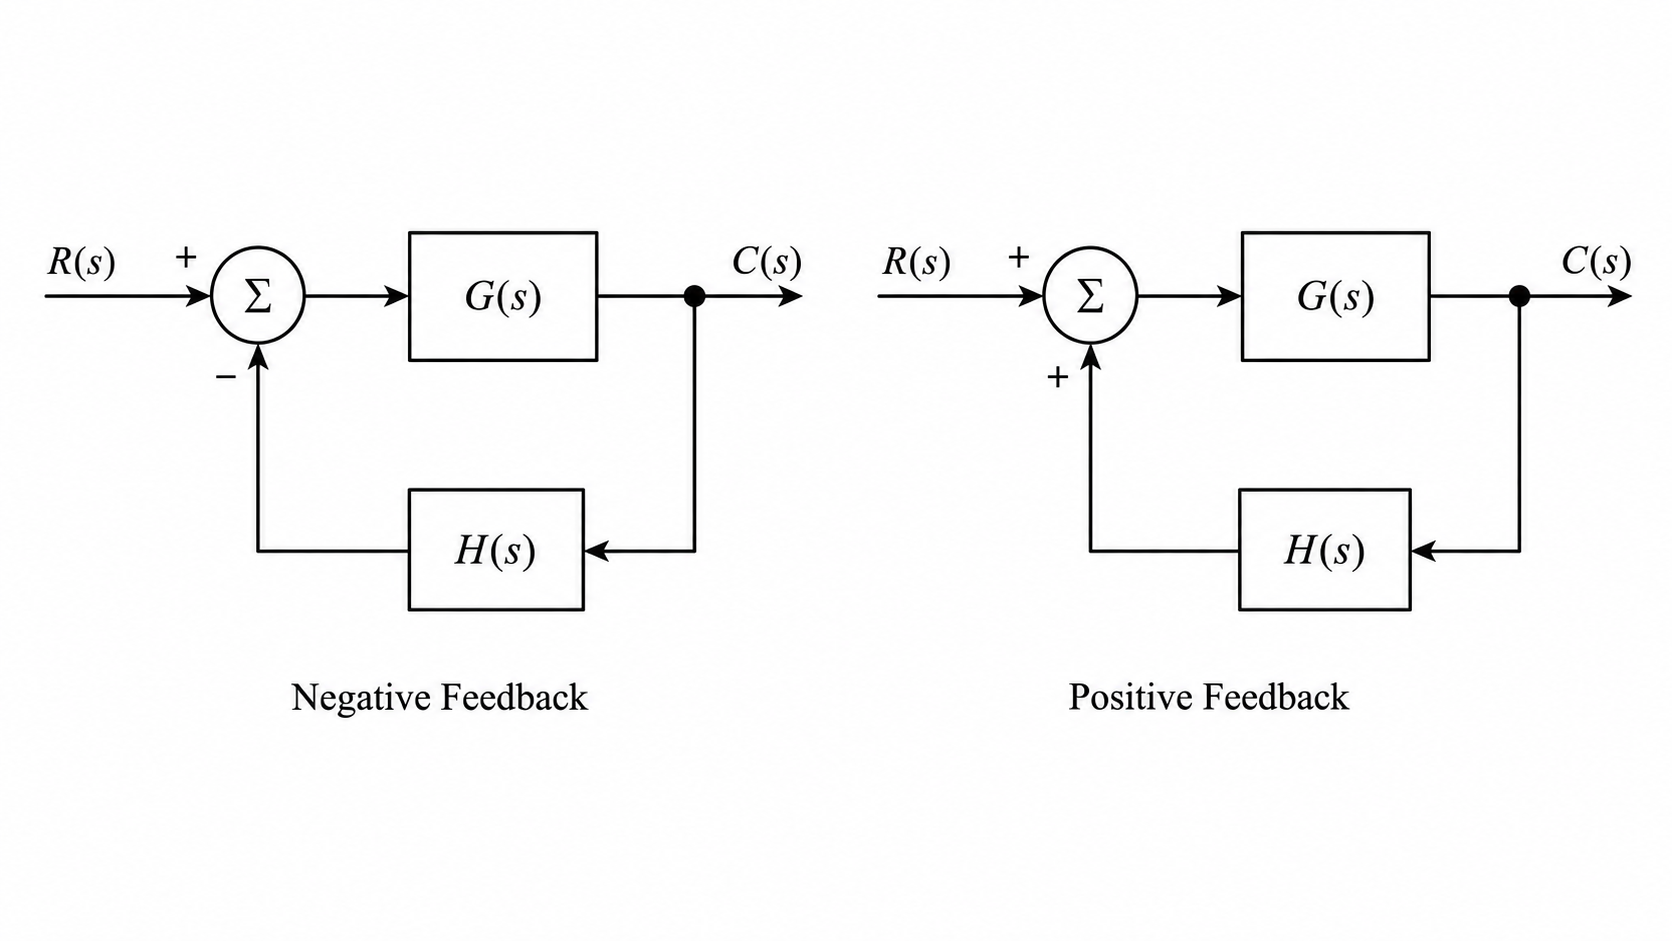
\includegraphics[width=0.8\textwidth]{images/chapter4/figure-03.png}
    \caption{โครงสร้างระบบป้อนกลับเชิงลบและเชิงบวก}
\end{figure}

\textbf{ตัวอย่างที่ 3: การป้อนกลับ (Feedback)}

\textbf{โจทย์:} ระบบควบคุมมีเส้นทางไปข้างหน้า $G(s) = \dfrac{10}{s+2}$ และเส้นทางป้อนกลับเชิงลบ $H(s) = 2$ จงหา closed-loop transfer function $C(s)/R(s)$

\textit{ขั้นตอนที่ 1–2 วิเคราะห์และกำหนดตัวแปร:} เป็นระบบป้อนกลับเชิงลบไม่ใช่หนึ่งหน่วย ($H(s) \neq 1$) สัญญาณผิดพลาด $E(s) = R(s) - H(s)C(s)$

\textit{ขั้นตอนที่ 3–4 เลือกกฎและสร้างสมการ:}

\[
\frac{C(s)}{R(s)} = \frac{G(s)}{1+G(s)H(s)} = \frac{\dfrac{10}{s+2}}{1 + \dfrac{10}{s+2}(2)}
\]

\textit{ขั้นตอนที่ 5–7 จัดรูปและคำนวณ:}

\[
\frac{C(s)}{R(s)} = \frac{\dfrac{10}{s+2}}{\dfrac{s+2+20}{s+2}} = \frac{10}{s+22}
\]

\textit{ขั้นตอนที่ 8 ตรวจสอบ:} ระบบเดิม (open-loop) เป็นระบบอันดับหนึ่งที่มีขั้ว (pole) ที่ $s=-2$ เมื่อปิดลูปป้อนกลับแล้วขั้วเลื่อนไปที่ $s=-22$ ซึ่งอยู่ไกลจากแกนจินตภาพมากขึ้น แสดงว่าระบบตอบสนองเร็วขึ้นเมื่อปิดลูป ซึ่งเป็นผลที่คาดได้จากการป้อนกลับเชิงลบที่มีอัตราขยายสูง

\textit{ขั้นตอนที่ 9 แปลความหมาย:} $\dfrac{C(s)}{R(s)} = \dfrac{10}{s+22}$ คือ closed-loop transfer function ของระบบ ซึ่งจะนำไปใช้วิเคราะห์การตอบสนองในบทที่ว่าด้วยการตอบสนองเชิงเวลา

\paragraph{7.3.4 การเลื่อนจุดรวมสัญญาณ (Moving Summing Junction)}

เมื่อจุดรวมสัญญาณอยู่คนละตำแหน่งกับบล็อกที่ต้องการรวม จำเป็นต้องเลื่อนจุดรวมสัญญาณผ่านบล็อกก่อนจึงจะใช้กฎอนุกรม/ขนาน/ป้อนกลับได้ หลักการคือ \textbf{ค่าที่ไหลผ่านจุดนั้นต้องไม่เปลี่ยนแปลง}

\begin{itemize}
    \item \textbf{เลื่อนจุดรวมสัญญาณไปด้านหลังบล็อก:} ต้องเพิ่มบล็อก $G(s)$ เข้าที่สัญญาณอีกเส้นที่เข้าจุดรวมสัญญาณนั้น เพื่อชดเชยผลของการย้าย
    \item \textbf{เลื่อนจุดรวมสัญญาณไปด้านหน้าบล็อก:} ต้องเพิ่มบล็อก $1/G(s)$ เข้าที่สัญญาณอีกเส้นแทน
\end{itemize}

% [รูปที่ 4: การเลื่อนจุดรวมสัญญาณไปด้านหน้าและด้านหลังบล็อก]
% ประเภทภาพ: Block Diagram
% ตำแหน่งที่แนะนำ: ท้ายหัวข้อ 7.3.4
% วัตถุประสงค์การเรียนรู้: แสดงว่าเมื่อเลื่อนจุดรวมสัญญาณผ่านบล็อก ต้องเพิ่มหรือหารด้วย $G(s)$ ที่สัญญาณอีกเส้นเพื่อให้ค่าที่จุดรวมสัญญาณเดิมไม่เปลี่ยนแปลง
% คำอธิบายภาพ: แถวบนแสดงบล็อก $G(s)$ ตามด้วยจุดรวมสัญญาณที่มีสัญญาณ $X(s)$ เข้ามาบวก แถวล่างแสดงจุดรวมสัญญาณย้ายมาก่อนบล็อก $G(s)$ พร้อมสัญญาณ $X(s)$ ที่ถูกส่งผ่านบล็อกเพิ่มเติม $1/G(s)$ ก่อนเข้าจุดรวมสัญญาณ เพื่อให้ผลลัพธ์เอาต์พุตเท่าเดิม
% องค์ประกอบที่ต้องมี: บล็อกสี่เหลี่ยม จุดรวมสัญญาณ บล็อกเสริม $1/G(s)$ หรือ $G(s)$ ลูกศรทิศทาง
% ข้อความหรือป้ายกำกับ: $G(s)$, $1/G(s)$, $X(s)$, เครื่องหมาย +
% ภาษาของป้ายกำกับ: ไทยและอังกฤษ
% สัดส่วนภาพ: 4:3
% Image Generation Prompt: Control systems block diagram equivalence pair showing a summing junction being moved across a block G(s): top diagram has block G(s) followed by a summing junction adding signal X(s); bottom equivalent diagram has the summing junction moved before block G(s), with signal X(s) now passed through an added block 1/G(s) before summation. Clean minimalist engineering diagram style, white background, black lines.
% Alt Text: ภาพแสดงกฎการเลื่อนจุดรวมสัญญาณผ่านบล็อกโดยต้องเพิ่มบล็อกชดเชย 1 ส่วน G(s)

\begin{figure}[htbp]
    \centering
    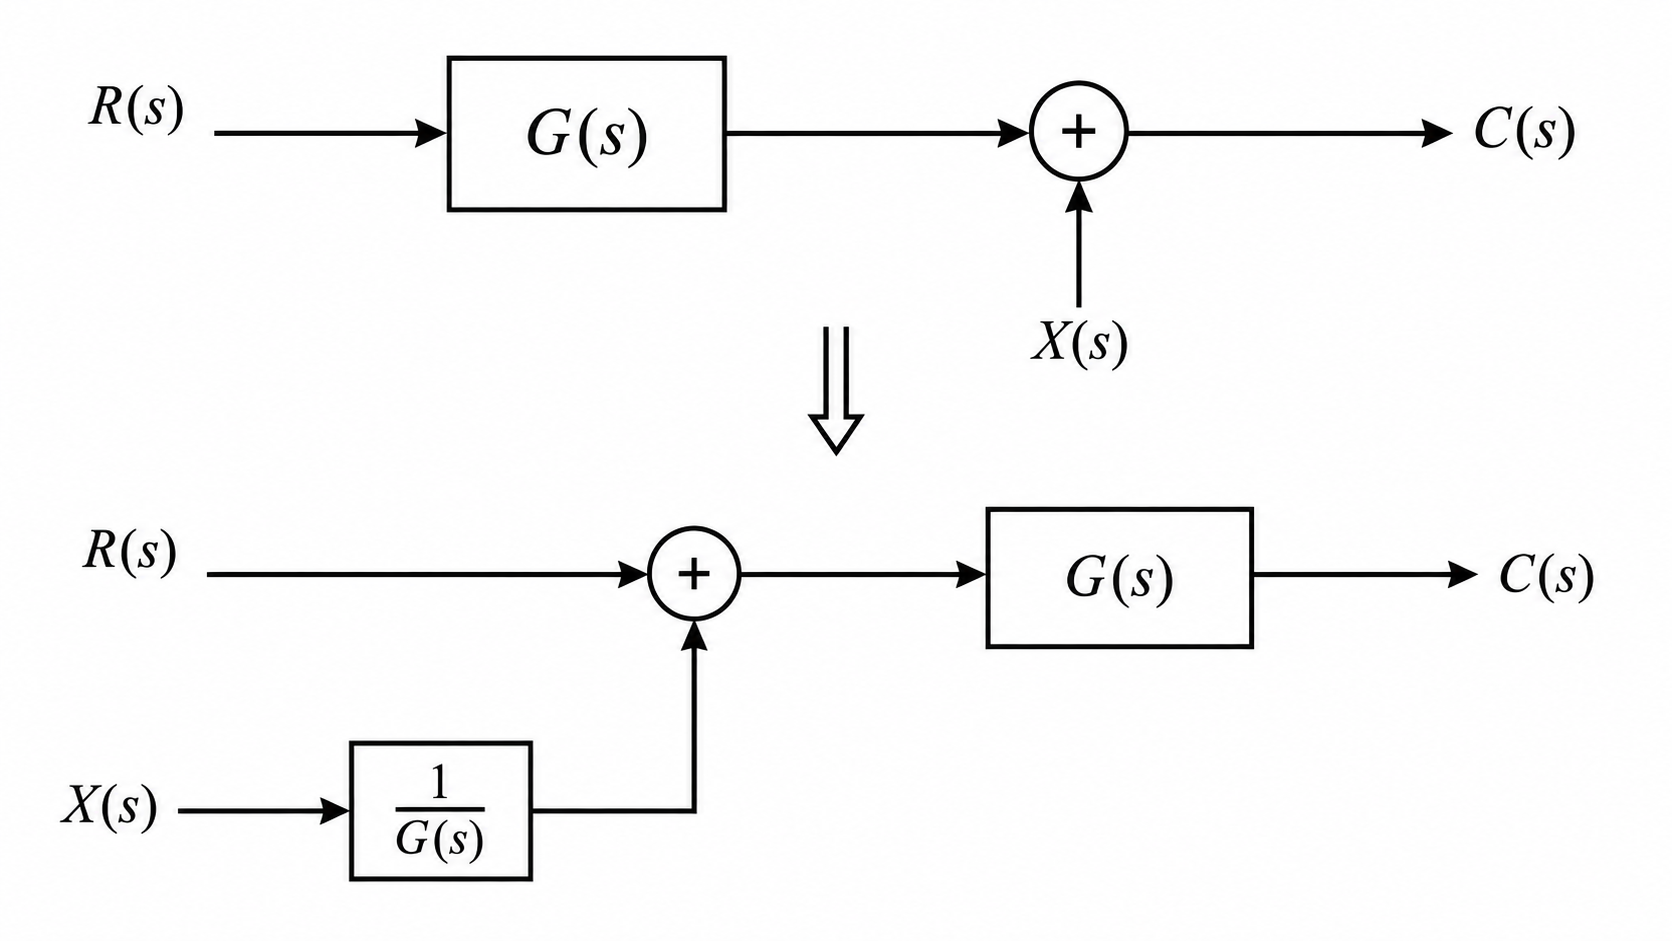
\includegraphics[width=0.8\textwidth]{images/chapter4/figure-04.png}
    \caption{การเลื่อนจุดรวมสัญญาณไปด้านหน้าและด้านหลังบล็อก}
\end{figure}

\paragraph{7.3.5 การเลื่อนจุดแยกสัญญาณ (Moving Takeoff Point)}

ในทำนองเดียวกัน เมื่อจุดแยกสัญญาณอยู่คนละตำแหน่งกับบล็อกที่ต้องการรวม สามารถเลื่อนได้โดยยังคงหลักการเดิมคือค่าที่แยกออกไปต้องไม่เปลี่ยนแปลง

\begin{itemize}
    \item \textbf{เลื่อนจุดแยกสัญญาณไปด้านหลังบล็อก:} ต้องเพิ่มบล็อก $1/G(s)$ เข้าที่เส้นสัญญาณที่แยกออกไป
    \item \textbf{เลื่อนจุดแยกสัญญาณไปด้านหน้าบล็อก:} ต้องเพิ่มบล็อก $G(s)$ เข้าที่เส้นสัญญาณที่แยกออกไปแทน
\end{itemize}

% [รูปที่ 5: การเลื่อนจุดแยกสัญญาณไปด้านหน้าและด้านหลังบล็อก]
% ประเภทภาพ: Block Diagram
% ตำแหน่งที่แนะนำ: ท้ายหัวข้อ 7.3.5
% วัตถุประสงค์การเรียนรู้: แสดงว่าเมื่อเลื่อนจุดแยกสัญญาณผ่านบล็อก ต้องเพิ่มบล็อกชดเชยที่เส้นแยกเพื่อรักษาค่าสัญญาณเดิม
% คำอธิบายภาพ: แถวบนแสดงบล็อก $G(s)$ แล้วจึงมีจุดแยกสัญญาณแยกเอาต์พุตออกไปเป็น $Y(s)$ แถวล่างแสดงจุดแยกสัญญาณย้ายมาก่อนบล็อก $G(s)$ พร้อมเพิ่มบล็อก $G(s)$ อีกตัวในเส้นที่แยกออกไปเพื่อให้ค่า $Y(s)$ เท่าเดิม
% องค์ประกอบที่ต้องมี: บล็อกสี่เหลี่ยม จุดแยกสัญญาณ บล็อกเสริม $G(s)$ หรือ $1/G(s)$ ลูกศรทิศทาง
% ข้อความหรือป้ายกำกับ: $G(s)$, $1/G(s)$, $Y(s)$
% ภาษาของป้ายกำกับ: ไทยและอังกฤษ
% สัดส่วนภาพ: 4:3
% Image Generation Prompt: Control systems block diagram equivalence pair showing a takeoff point being moved across a block G(s): top diagram has block G(s) followed by a takeoff point branching signal Y(s); bottom equivalent diagram has the takeoff point moved before block G(s), with an added block G(s) inserted in the branched line so Y(s) stays identical. Clean minimalist engineering diagram style, white background, black lines.
% Alt Text: ภาพแสดงกฎการเลื่อนจุดแยกสัญญาณผ่านบล็อกโดยต้องเพิ่มบล็อกชดเชย G(s)

\begin{figure}[htbp]
    \centering
    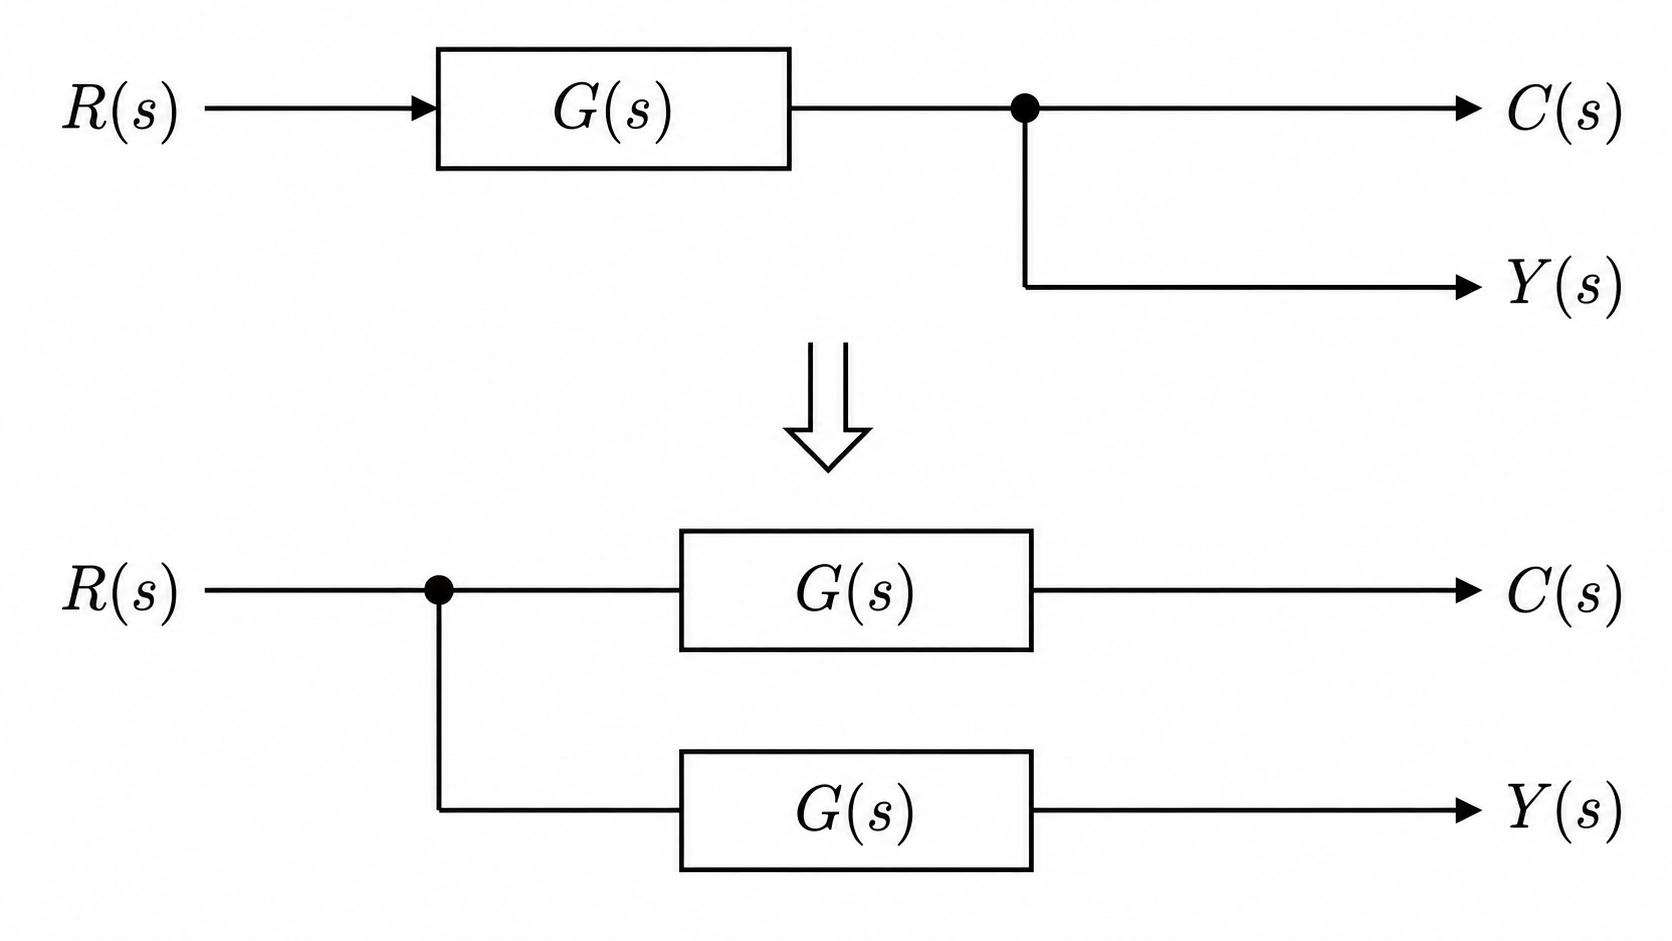
\includegraphics[width=0.8\textwidth]{images/chapter4/figure-05.png}
    \caption{การเลื่อนจุดแยกสัญญาณไปด้านหน้าและด้านหลังบล็อก}
\end{figure}


\textbf{ตารางที่ 3} สรุปกฎการลดรูปแผนภาพบล็อกที่ใช้บ่อย

\begin{table}[htbp]
    \centering
    \begin{tabularx}{\textwidth}{L{0.23\textwidth} Y Y}
        \hline
        \textbf{กฎ} & \textbf{โครงสร้างเดิม} & \textbf{ผลลัพธ์หลังลดรูป} \\
        \hline
        การต่อแบบอนุกรม & $G_1(s)$ ตามด้วย $G_2(s)$ & $G_1(s)G_2(s)$ \\
        การต่อแบบขนาน & $G_1(s)$ และ $G_2(s)$ รับอินพุตเดียวกัน บวกที่เอาต์พุต & $G_1(s) \pm G_2(s)$ \\
        การป้อนกลับเชิงลบ & $G(s)$ ในเส้นไปข้างหน้า, $H(s)$ ป้อนกลับลบ & $\dfrac{G(s)}{1+G(s)H(s)}$ \\
        การป้อนกลับเชิงบวก & $G(s)$ ในเส้นไปข้างหน้า, $H(s)$ ป้อนกลับบวก & $\dfrac{G(s)}{1-G(s)H(s)}$ \\
        เลื่อนจุดรวมสัญญาณไปด้านหลังบล็อก & จุดรวมสัญญาณอยู่หน้าบล็อก $G(s)$ & เพิ่มบล็อก $G(s)$ ที่สัญญาณอีกเส้น \\
        เลื่อนจุดรวมสัญญาณไปด้านหน้าบล็อก & จุดรวมสัญญาณอยู่หลังบล็อก $G(s)$ & เพิ่มบล็อก $1/G(s)$ ที่สัญญาณอีกเส้น \\
        เลื่อนจุดแยกสัญญาณไปด้านหลังบล็อก & จุดแยกสัญญาณอยู่หน้าบล็อก $G(s)$ & เพิ่มบล็อก $1/G(s)$ ที่เส้นแยก \\
        เลื่อนจุดแยกสัญญาณไปด้านหน้าบล็อก & จุดแยกสัญญาณอยู่หลังบล็อก $G(s)$ & เพิ่มบล็อก $G(s)$ ที่เส้นแยก \\
        \hline
    \end{tabularx}
\end{table}


\subsubsection{7.4 ขั้นตอนการลดรูปแผนภาพบล็อกที่มีหลายลูปซ้อนกัน}

ระบบควบคุมจริงมักมีลูปป้อนกลับซ้อนกันหลายชั้น (multiple nested loops) ซึ่งไม่สามารถใช้กฎอนุกรม ขนาน หรือป้อนกลับได้ทันทีเพราะมีจุดรวมสัญญาณหรือจุดแยกสัญญาณคั่นอยู่ระหว่างบล็อก แนวทางที่แนะนำสำหรับการลดรูปแผนภาพบล็อกที่ซับซ้อนมีลำดับขั้นตอนดังนี้

\begin{enumerate}
    \item \textbf{รวมบล็อกอนุกรมและขนานที่ไม่มีจุดรวม/จุดแยกสัญญาณคั่นกลาง} ให้เหลือน้อยบล็อกที่สุดก่อน
    \item \textbf{เลื่อนจุดรวมสัญญาณหรือจุดแยกสัญญาณ} (ตามหัวข้อ 7.3.4–7.3.5) เพื่อให้จุดรวม/จุดแยกสัญญาณที่ขวางอยู่เคลื่อนออกจากลูปด้านใน
    \item \textbf{ลดรูปลูปป้อนกลับที่อยู่ด้านในสุดก่อน} โดยใช้สูตร $G/(1\pm GH)$ แล้วแทนที่ลูปนั้นด้วยบล็อกสมมูลบล็อกเดียว
    \item \textbf{ทำซ้ำขั้นตอนที่ 1–3} จากลูปในสุดไล่ออกไปยังลูปนอกสุด จนเหลือแผนภาพที่มีเพียงเส้นทางไปข้างหน้าเส้นเดียวกับลูปป้อนกลับหลักเพียงลูปเดียว
    \item \textbf{ใช้กฎการป้อนกลับ} ลดรูปลูปสุดท้ายให้เหลือบล็อกเดียว ซึ่งคือ transfer function รวมของทั้งระบบ
\end{enumerate}

ข้อควรระวังที่สำคัญคือ \textbf{ควรลดรูปลูปในสุดก่อนเสมอ} และหลีกเลี่ยงการเลื่อนจุดรวมสัญญาณผ่านจุดแยกสัญญาณ (หรือในทางกลับกัน) เนื่องจากลำดับการดำเนินการทั้งสองไม่สามารถสลับกันได้โดยทั่วไป หากแผนภาพมีจุดรวมสัญญาณและจุดแยกสัญญาณสลับซับซ้อนกันมาก ควรพิจารณาแปลงเป็น Signal Flow Graph และใช้ Mason's Gain Formula แทน ซึ่งจะกล่าวถึงในหัวข้อถัดไป

\subsubsection{7.5 Signal Flow Graph (SFG)}

\textbf{Signal Flow Graph (SFG)} เป็นอีกแนวทางหนึ่งในการแทนความสัมพันธ์เชิงเส้นระหว่างตัวแปรของระบบด้วยกราฟทิศทาง (directed graph) แทนที่จะใช้บล็อกสี่เหลี่ยมและจุดรวม/จุดแยกสัญญาณแบบ Block Diagram โดยทุกความสัมพันธ์เชิงเส้นสามารถแปลงเป็น SFG ได้เสมอ และทุก SFG สามารถแปลงกลับเป็น Block Diagram ได้เช่นกัน ข้อได้เปรียบสำคัญของ SFG คือสามารถหา transfer function รวมได้โดยตรงจากโครงสร้างกราฟด้วย \textbf{Mason's Gain Formula} โดยไม่ต้องลดรูปทีละขั้นตอนเหมือน Block Diagram

\paragraph{7.5.1 Node และ Branch}

\begin{itemize}
    \item \textbf{โหนด (Node):} จุดที่แทนตัวแปรหรือสัญญาณหนึ่งตัวในระบบ เช่น $R(s)$, $E(s)$, $C(s)$ ค่าของโหนดหนึ่งเท่ากับผลรวมของสัญญาณทั้งหมดที่ไหลเข้าสู่โหนดนั้นตามกิ่งที่เชื่อมเข้ามา
    \item \textbf{กิ่ง (Branch):} เส้นเชื่อมมีทิศทางระหว่างสองโหนด กำกับด้วยค่าอัตราขยาย (gain หรือ transmittance) ของกิ่งนั้น สัญญาณที่โหนดปลายทางเท่ากับสัญญาณที่โหนดต้นทางคูณด้วยอัตราขยายของกิ่ง
\end{itemize}

\paragraph{7.5.2 Path และ Forward Path}

\begin{itemize}
    \item \textbf{เส้นทาง (Path):} ลำดับของกิ่งที่เชื่อมต่อกันตามทิศทางลูกศรอย่างต่อเนื่องโดยไม่ผ่านโหนดใดซ้ำ
    \item \textbf{เส้นทางหน้า (Forward Path):} เส้นทางที่เริ่มจากโหนดอินพุต (source node) ไปสิ้นสุดที่โหนดเอาต์พุต (sink node) โดยไม่ผ่านโหนดใดซ้ำ อัตราขยายของเส้นทางหน้า ($P_k$) คือผลคูณของอัตราขยายกิ่งทั้งหมดที่ประกอบเป็นเส้นทางนั้น
\end{itemize}

\paragraph{7.5.3 Loop และ Loop Gain}

\textbf{ลูป (Loop):} เส้นทางปิดที่เริ่มต้นและสิ้นสุดที่โหนดเดียวกัน โดยไม่ผ่านโหนดอื่นซ้ำระหว่างทาง \textbf{อัตราขยายลูป (Loop Gain)} คือผลคูณของอัตราขยายกิ่งทั้งหมดที่ประกอบเป็นลูปนั้น

\paragraph{7.5.4 Non-touching Loop}

ลูปตั้งแต่สองลูปขึ้นไปเรียกว่า \textbf{ลูปไม่สัมผัสกัน (Non-touching Loop)} เมื่อลูปเหล่านั้น\textbf{ไม่มีโหนดร่วมกันเลย} แนวคิดนี้เป็นหัวใจสำคัญของ Mason's Gain Formula เนื่องจากค่าดีเทอร์มิแนนต์ของกราฟต้องคำนึงถึงผลคูณของอัตราขยายของลูปที่ไม่สัมผัสกันด้วย ในทางกลับกัน หากเส้นทางหน้าหรือลูปใดมีโหนดร่วมกับลูปอื่น จะเรียกว่า\textbf{สัมผัสกัน (touching)}

% [รูปที่ 6: Signal Flow Graph แสดง Node, Branch, Forward Path และ Loop]
% ประเภทภาพ: Technical Illustration
% ตำแหน่งที่แนะนำ: ท้ายหัวข้อ 7.5.4
% วัตถุประสงค์การเรียนรู้: ให้ผู้เรียนระบุ Node, Branch, Forward Path และ Loop บน Signal Flow Graph ได้ถูกต้อง
% คำอธิบายภาพ: แสดงกราฟที่มีโหนดเรียงจากซ้ายไปขวา ได้แก่ $R$, $1$, $2$, $3$, $C$ เชื่อมด้วยกิ่งกำกับอัตราขยาย $G_1$, $G_2$, $G_3$ ตามลำดับ (เส้นทางหน้า) และมีกิ่งย้อนกลับจากโหนด 2 กลับไปโหนด 1 กำกับด้วย $-H_1$ แสดงเป็นลูป วงกลมประแนวเส้นทางหน้าด้วยสีหนึ่ง และวงกลมลูปด้วยเส้นประอีกสีหนึ่ง พร้อมป้ายกำกับ "Forward Path" และ "Loop"
% องค์ประกอบที่ต้องมี: โหนดวงกลมเล็ก 5 โหนด กิ่งลูกศรกำกับอัตราขยาย กิ่งย้อนกลับแสดงลูป เส้นประเน้นเส้นทางหน้าและลูป ป้ายกำกับภาษาไทย/อังกฤษ
% ข้อความหรือป้ายกำกับ: $R$, $C$, $G_1$, $G_2$, $G_3$, $-H_1$, "Forward Path", "Loop"
% ภาษาของป้ายกำกับ: ไทยและอังกฤษ
% สัดส่วนภาพ: 16:9
% Image Generation Prompt: Signal flow graph diagram for a control systems textbook: five small circular nodes labeled R, 1, 2, 3, C arranged left to right, connected by directed arrows (branches) labeled G1, G2, G3 forming the main chain, plus one feedback arrow curving from node 2 back to node 1 labeled -H1 forming a loop. Highlight the forward path chain with a dashed overlay labeled "Forward Path" and the feedback loop with a different dashed overlay labeled "Loop". Clean minimalist black-and-white engineering diagram, white background.
% Alt Text: ภาพกราฟการไหลของสัญญาณแสดงโหนด กิ่ง เส้นทางหน้า และลูปป้อนกลับ

\begin{figure}[htbp]
    \centering
    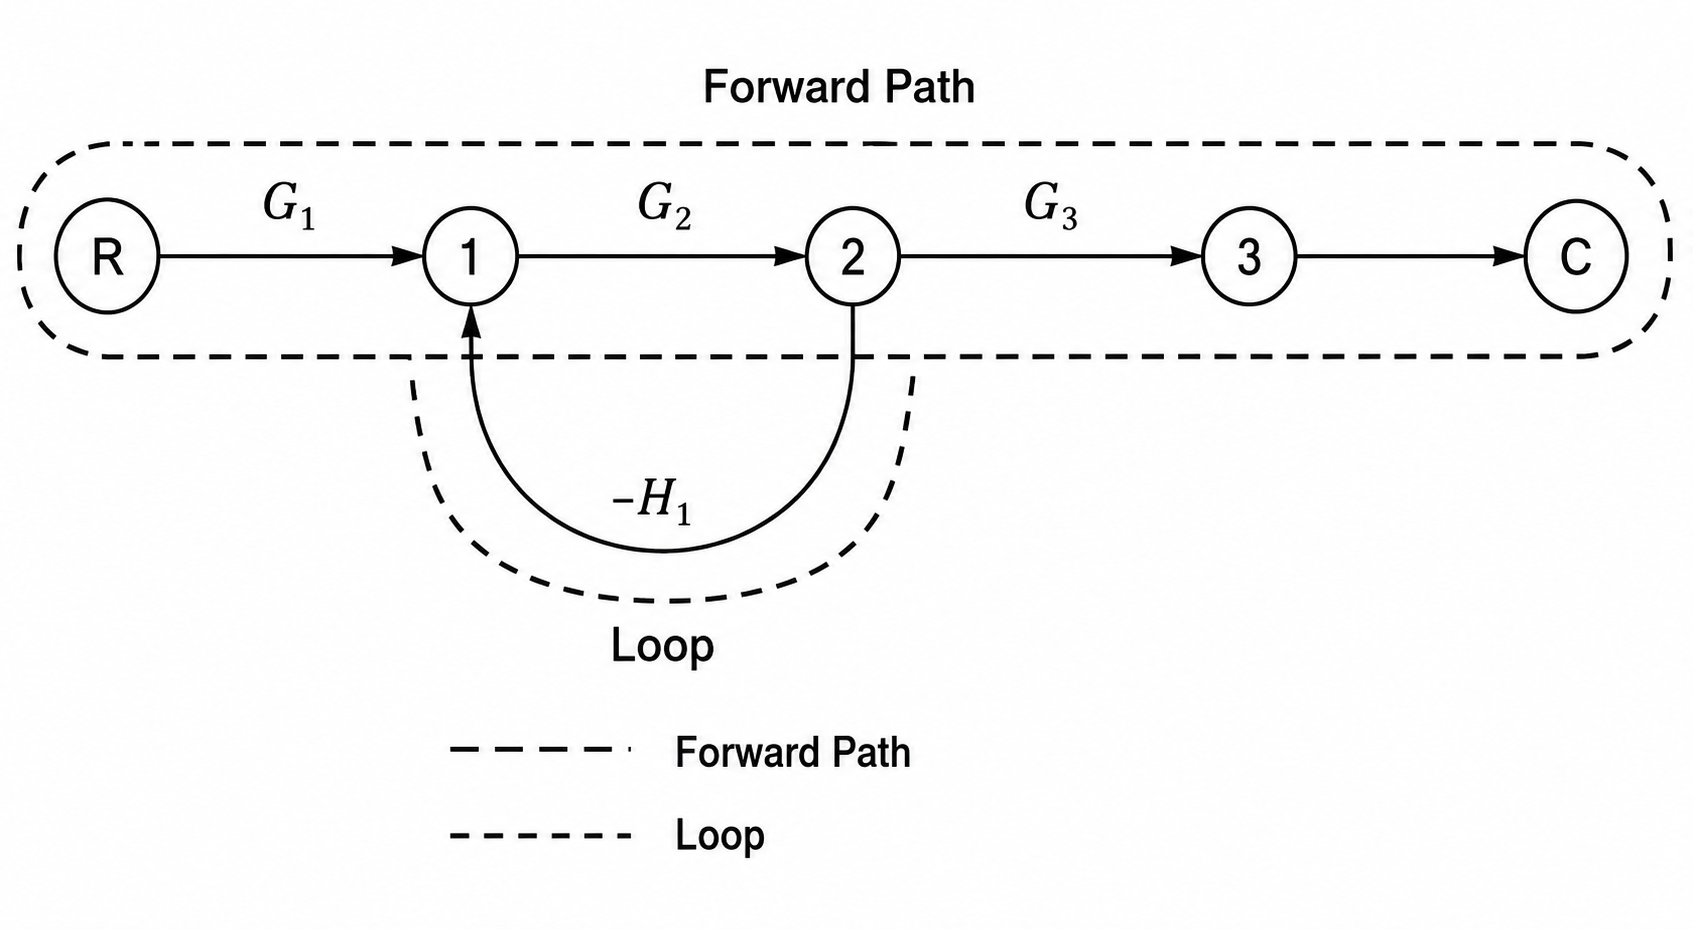
\includegraphics[width=0.8\textwidth]{images/chapter4/figure-06.png}
    \caption{Signal Flow Graph แสดง Node, Branch, Forward Path และ Loop}
\end{figure}

\subsubsection{7.6 Mason's Gain Formula}

\textbf{Mason's Gain Formula} เป็นสูตรที่ใช้คำนวณอัตราขยายรวม (overall transfer function) ระหว่างโหนดอินพุตกับโหนดเอาต์พุตของ Signal Flow Graph ได้โดยตรงจากโครงสร้างกราฟ โดยไม่ต้องลดรูปทีละขั้นตอน สูตรมีรูปแบบดังนี้

\[
P = \frac{C(s)}{R(s)} = \frac{1}{\Delta}\sum_{k} P_k \, \Delta_k
\]

โดยที่

\begin{itemize}
    \item $P$ คือ transfer function รวมระหว่างโหนดอินพุตกับโหนดเอาต์พุต
    \item $P_k$ คืออัตราขยายของเส้นทางหน้าเส้นที่ $k$
    \item $\Delta$ คือ \textbf{ดีเทอร์มิแนนต์ของกราฟ (graph determinant)} คำนวณจาก
\end{itemize}

\[
\Delta = 1 - \sum L_i + \sum L_iL_j - \sum L_iL_jL_k + \cdots
\]

โดย $\sum L_i$ คือผลรวมของอัตราขยายลูปทั้งหมด $\sum L_iL_j$ คือผลรวมของผลคูณอัตราขยายของทุกคู่ลูปที่ไม่สัมผัสกัน $\sum L_iL_jL_k$ คือผลรวมของผลคูณอัตราขยายของทุกกลุ่มสามลูปที่ไม่สัมผัสกัน และเป็นเช่นนี้ต่อไปสำหรับกลุ่มลูปที่ไม่สัมผัสกันจำนวนมากขึ้น

\begin{itemize}
    \item $\Delta_k$ คือ \textbf{โคแฟกเตอร์ของเส้นทางหน้าที่ $k$ (path cofactor)} ซึ่งคำนวณเหมือน $\Delta$ แต่พิจารณาเฉพาะส่วนของกราฟที่\textbf{ไม่สัมผัส}กับเส้นทางหน้าที่ $k$ นั้น กล่าวคือ ตัดลูปทุกลูปที่มีโหนดร่วมกับเส้นทางหน้าที่ $k$ ออกก่อนคำนวณ
\end{itemize}

\textbf{ขั้นตอนการคำนวณด้วย Mason's Gain Formula}

\begin{enumerate}
    \item เขียน Signal Flow Graph ของระบบให้ครบถ้วน กำกับอัตราขยายทุกกิ่ง
    \item ระบุเส้นทางหน้าทั้งหมดและคำนวณอัตราขยาย $P_k$ ของแต่ละเส้นทาง
    \item ระบุลูปทั้งหมดในกราฟและคำนวณอัตราขยายลูปแต่ละลูป
    \item ตรวจสอบคู่ กลุ่มสาม ฯลฯ ของลูปที่ไม่สัมผัสกัน (ไม่มีโหนดร่วมกัน)
    \item คำนวณดีเทอร์มิแนนต์ $\Delta$ จากผลรวมและผลคูณตามสูตร
    \item คำนวณโคแฟกเตอร์ $\Delta_k$ ของแต่ละเส้นทางหน้า โดยตัดลูปที่สัมผัสกับเส้นทางนั้นออก
    \item แทนค่า $P_k$ และ $\Delta_k$ ลงในสูตรและรวมผลทุกเส้นทาง แล้วหารด้วย $\Delta$
    \item จัดรูปและตรวจสอบผลลัพธ์ให้อยู่ในรูป transfer function ที่เป็นเศษส่วนของพหุนามใน $s$
\end{enumerate}


% [รูปที่ 7: Signal Flow Graph สำหรับตัวอย่างที่ 4 การประยุกต์ใช้ Mason's Gain Formula]
% ประเภทภาพ: Technical Illustration
% ตำแหน่งที่แนะนำ: ก่อนตัวอย่างที่ 4
% วัตถุประสงค์การเรียนรู้: ให้ผู้เรียนเห็นโครงสร้างกราฟที่มีสองเส้นทางหน้าและสองลูปไม่สัมผัสกัน ก่อนฝึกคำนวณด้วย Mason's Gain Formula
% คำอธิบายภาพ: แสดงโหนด $R$, $1$, $2$, $3$, $4$, $5$, $C$ โดยเส้นทางหน้าที่หนึ่งไหลจาก $R \to 1 \to 2 \to 3 \to 4 \to C$ กำกับอัตราขยาย $G_1, G_2, G_3, G_4, G_5$ ตามลำดับ เส้นทางหน้าที่สองไหลจาก $R \to 5 \to 4 \to C$ กำกับอัตราขยาย $G_6, G_7, G_5$ มีลูป $L_1$ จากโหนด 2 กลับไปโหนด 1 กำกับ $-H_1$ และลูป $L_2$ จากโหนด 4 กลับไปโหนด 3 กำกับ $-H_2$ ระบายสีหรือเส้นประแยกลูปทั้งสองให้เห็นชัดว่าไม่มีโหนดร่วมกัน
% องค์ประกอบที่ต้องมี: โหนด 7 โหนด กิ่งกำกับอัตราขยายครบทุกกิ่ง ลูกศรทิศทาง เส้นประหรือสีแยกลูป $L_1$ และ $L_2$
% ข้อความหรือป้ายกำกับ: $R$, $C$, $1$-$5$, $G_1$-$G_7$, $-H_1$, $-H_2$
% ภาษาของป้ายกำกับ: ไทยและอังกฤษ
% สัดส่วนภาพ: 16:9
% Image Generation Prompt: Signal flow graph for a control systems worked example: nodes R, 1, 2, 3, 4, 5, C. Main chain forward path R-1-2-3-4-C with branch gains G1, G2, G3, G4, G5. Second forward path R-5-4-C with branch gains G6, G7 feeding into node 4 then G5 to C. A feedback loop from node 2 back to node 1 labeled -H1, and a separate feedback loop from node 4 back to node 3 labeled -H2, drawn with distinct dashed colors to show they share no common nodes. Clean minimalist black-and-white engineering diagram, white background, clear labels.
% Alt Text: ภาพกราฟการไหลของสัญญาณที่มีสองเส้นทางหน้าและสองลูปป้อนกลับที่ไม่สัมผัสกัน ใช้ประกอบตัวอย่างการคำนวณด้วยสูตรเมสัน

\begin{figure}[htbp]
    \centering
    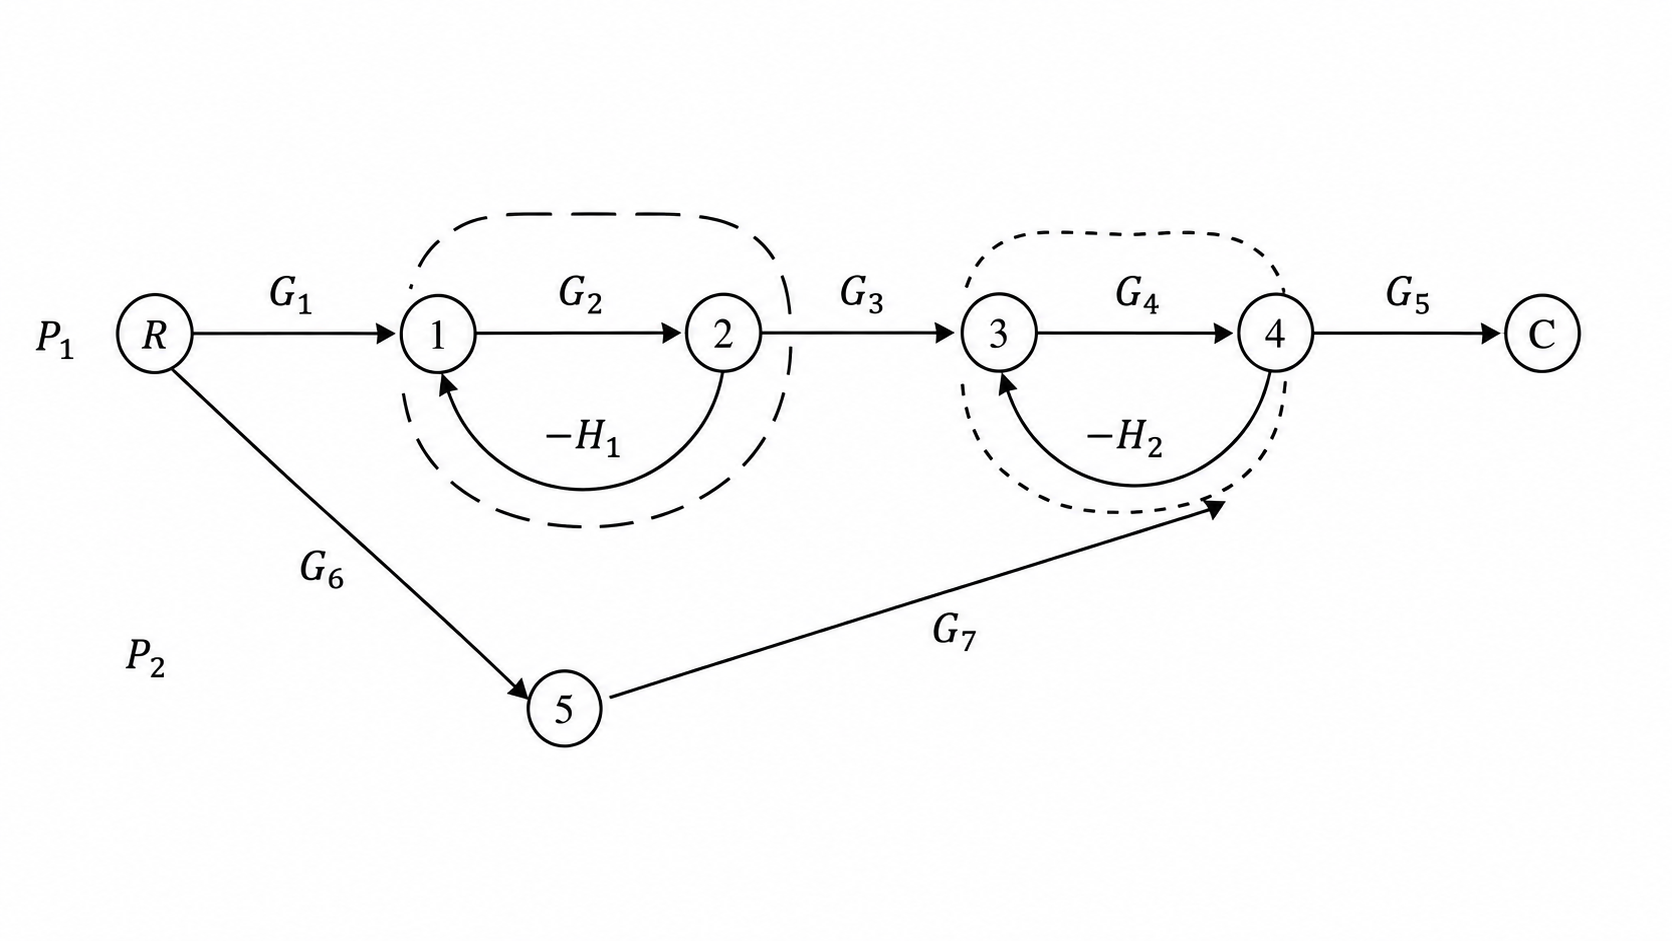
\includegraphics[width=0.8\textwidth]{images/chapter4/figure-07.png}
    \caption{Signal Flow Graph สำหรับตัวอย่างที่ 4 การประยุกต์ใช้ Mason's Gain Formula}
\end{figure}

\textbf{ตัวอย่างที่ 4: การประยุกต์ใช้ Mason's Gain Formula}

\textbf{โจทย์:} Signal Flow Graph ของระบบหนึ่งมีโหนดอินพุต $R$ และโหนดเอาต์พุต $C$ ประกอบด้วย

\begin{itemize}
    \item เส้นทางหน้าที่ 1: $R \to 1 \to 2 \to 3 \to 4 \to C$ อัตราขยายกิ่งตามลำดับคือ $G_1, G_2, G_3, G_4, G_5$
    \item เส้นทางหน้าที่ 2: $R \to 5 \to 4 \to C$ อัตราขยายกิ่งตามลำดับคือ $G_6, G_7$ (เข้าสู่โหนด 4) แล้วออกด้วยกิ่งเดิม $G_5$
    \item ลูป $L_1$: จากโหนด 2 กลับไปโหนด 1 อัตราขยาย $-H_1$ (ประกอบด้วยกิ่ง $G_2$ และกิ่งย้อนกลับ $-H_1$)
    \item ลูป $L_2$: จากโหนด 4 กลับไปโหนด 3 อัตราขยาย $-H_2$ (ประกอบด้วยกิ่ง $G_4$ และกิ่งย้อนกลับ $-H_2$)
\end{itemize}

จงหา transfer function รวม $C(s)/R(s)$ ด้วย Mason's Gain Formula

\textit{ขั้นตอนที่ 1 เขียน SFG:} ตามรูปที่ 7

\textit{ขั้นตอนที่ 2 ระบุเส้นทางหน้าและคำนวณ $P_k$:}

\[
P_1 = G_1G_2G_3G_4G_5, \qquad P_2 = G_6G_7G_5
\]

\textit{ขั้นตอนที่ 3 ระบุลูปและคำนวณอัตราขยายลูป:}

ลูป $L_1$ ประกอบด้วยกิ่ง $1\to2$ (อัตราขยาย $G_2$) และกิ่งย้อนกลับ $2\to1$ (อัตราขยาย $-H_1$) ดังนั้นอัตราขยายลูปคือ

\[
L_1 = G_2(-H_1) = -G_2H_1
\]

ลูป $L_2$ ประกอบด้วยกิ่ง $3\to4$ (อัตราขยาย $G_4$) และกิ่งย้อนกลับ $4\to3$ (อัตราขยาย $-H_2$) ดังนั้น

\[
L_2 = G_4(-H_2) = -G_4H_2
\]

\textit{ขั้นตอนที่ 4 ตรวจสอบลูปที่ไม่สัมผัสกัน:} $L_1$ ใช้โหนด $\{1,2\}$ และ $L_2$ ใช้โหนด $\{3,4\}$ ไม่มีโหนดร่วมกัน จึงเป็น \textbf{ลูปไม่สัมผัสกัน} หนึ่งคู่

\textit{ขั้นตอนที่ 5 คำนวณดีเทอร์มิแนนต์ $\Delta$:}

\[
\Delta = 1 - (L_1+L_2) + (L_1L_2) = 1-(-G_2H_1-G_4H_2)+(-G_2H_1)(-G_4H_2)
\]

\[
\Delta = 1 + G_2H_1 + G_4H_2 + G_2H_1G_4H_2
\]

\textit{ขั้นตอนที่ 6 คำนวณโคแฟกเตอร์ $\Delta_k$ ของแต่ละเส้นทางหน้า:}

เส้นทางหน้าที่ 1 ผ่านโหนด $\{1,2,3,4\}$ ซึ่งสัมผัสทั้ง $L_1$ (โหนด 1,2) และ $L_2$ (โหนด 3,4) จึงไม่เหลือลูปใดที่ไม่สัมผัสกับเส้นทางนี้

\[
\Delta_1 = 1
\]

เส้นทางหน้าที่ 2 ผ่านโหนด $\{5,4\}$ เท่านั้น สัมผัสกับ $L_2$ (มีโหนด 4 ร่วมกัน) แต่\textbf{ไม่สัมผัส}กับ $L_1$ (ไม่มีโหนดร่วมกับ $\{1,2\}$) ดังนั้นเมื่อคำนวณ $\Delta_2$ ต้องคงเฉพาะลูปที่ไม่สัมผัสกับเส้นทางที่ 2 ไว้ คือ $L_1$

\[
\Delta_2 = 1 - L_1 = 1-(-G_2H_1) = 1+G_2H_1
\]

\textit{ขั้นตอนที่ 7 แทนค่าในสูตรเมสัน:}

\[
\frac{C(s)}{R(s)} = \frac{P_1\Delta_1 + P_2\Delta_2}{\Delta} = \frac{G_1G_2G_3G_4G_5(1) + G_6G_7G_5(1+G_2H_1)}{1+G_2H_1+G_4H_2+G_2H_1G_4H_2}
\]

\textit{ขั้นตอนที่ 8 ตรวจสอบและแปลความหมาย:} สังเกตว่า $\Delta_1 = 1$ เนื่องจากเส้นทางหน้าที่ 1 ผ่านทุกโหนดที่เกี่ยวข้องกับทั้งสองลูป จึงไม่มีลูปใดเหลือให้พิจารณาเป็นพิเศษ ในขณะที่ $\Delta_2 \neq 1$ เพราะเส้นทางหน้าที่ 2 "ข้าม" ลูป $L_1$ ไปโดยไม่ผ่านโหนด 1 และ 2 เลย ทำให้ $L_1$ ยังคงมีผลต่อโคแฟกเตอร์ของเส้นทางนี้ นี่คือใจความสำคัญที่ทำให้ต้องแยกพิจารณา $\Delta_k$ ของแต่ละเส้นทางหน้าอย่างระมัดระวัง มิใช่ใช้ $\Delta$ เดียวกันกับทุกเส้นทาง

เพื่อยืนยันความสมเหตุสมผลของสูตร ลองแทนค่าตัวเลข: กำหนดให้ $G_1=G_2=G_3=G_6=G_7=1$, $G_4=2$, $G_5=1$, $H_1=1$, $H_2=1$ จะได้ $\Delta = 1+1+2+2 = 6$, $P_1\Delta_1 = (1)(1)(1)(2)(1)(1)=2$, $P_2\Delta_2 = (1)(1)(1)(1+1) = 2$ ดังนั้น $C(s)/R(s) = (2+2)/6 = 2/3$ ซึ่งเป็นค่าคงที่ที่ตรวจสอบย้อนกลับได้ด้วยการลดรูปแผนภาพบล็อกทีละขั้นตอนเช่นกัน แสดงให้เห็นว่าทั้งสองวิธีให้ผลลัพธ์ตรงกัน

\subsubsection{7.7 การเปรียบเทียบ Block Diagram Reduction กับ Signal Flow Graph}

\textbf{ตารางที่ 4} เปรียบเทียบข้อดีและข้อจำกัดของทั้งสองวิธี

\begin{table}[htbp]
    \centering
    \small
    \begin{tabularx}{\textwidth}{L{0.18\textwidth} Y Y}
        \hline
        \textbf{ประเด็น} & \textbf{Block Diagram Reduction} & \textbf{Signal Flow Graph + Mason's Gain Formula} \\
        \hline
        ความเข้าใจเชิงภาพ & เห็นโครงสร้างระบบและเส้นทางสัญญาณได้ชัดเจน เหมาะสำหรับสื่อสารการออกแบบ & เข้าใจยากกว่าในระบบง่าย เนื่องจากใช้โหนดและกิ่งแทนบล็อก \\
        ความเหมาะสมกับระบบซับซ้อน & ต้องลดรูปหลายขั้นตอน เสี่ยงต่อความผิดพลาดเมื่อมีหลายลูปซ้อนกัน & คำนวณได้โดยตรงจากโครงสร้างกราฟโดยไม่ต้องลดรูปทีละขั้น เหมาะกับระบบที่มีหลายลูป \\
        ความเสี่ยงต่อข้อผิดพลาด & มีโอกาสผิดพลาดจากการเลื่อนจุดรวม/จุดแยกสัญญาณผิดลำดับ & มีโอกาสผิดพลาดจากการระบุลูปหรือคู่ลูปไม่สัมผัสกันไม่ครบถ้วน \\
        ความเหมาะสมกับผู้เริ่มต้น & เข้าใจง่ายกว่าในช่วงเริ่มต้น เพราะใช้กฎพีชคณิตที่คุ้นเคย & ต้องฝึกฝนการระบุองค์ประกอบของกราฟให้คล่องก่อนจึงจะใช้ได้อย่างมีประสิทธิภาพ \\
        การใช้งานร่วมกับซอฟต์แวร์ & MATLAB มีคำสั่ง \texttt{series}, \texttt{parallel}, \texttt{feedback} รองรับโดยตรง & MATLAB ไม่มีคำสั่งสำหรับ SFG โดยตรง มักใช้ตรวจผลด้วยการแปลงเป็น Block Diagram หรือ state-space ก่อน \\
        \hline
    \end{tabularx}
\end{table}

โดยสรุป ทั้งสองวิธีให้ผลลัพธ์ transfer function เดียวกันเสมอเมื่อคำนวณถูกต้อง การเลือกใช้วิธีใดขึ้นอยู่กับโครงสร้างของระบบและความถนัดของผู้ใช้งาน สำหรับระบบที่มีลูปป้อนกลับไม่มากและไม่ซ้อนกันซับซ้อน การลดรูปแผนภาพบล็อกทีละขั้นตอนมักสะดวกและตรวจสอบได้ง่ายกว่า ในขณะที่ระบบที่มีหลายลูปซ้อนกันหรือมีเส้นทางหน้าหลายเส้นทาง การใช้ Signal Flow Graph ร่วมกับ Mason's Gain Formula มักลดความซับซ้อนและข้อผิดพลาดได้มากกว่า


\subsubsection{7.8 การใช้ MATLAB และ Simulink ยืนยันผลการลดรูป}

MATLAB มีคำสั่งในกลุ่ม Control System Toolbox ที่รองรับการรวม transfer function ตามกฎการลดรูปแผนภาพบล็อกโดยตรง ได้แก่ \texttt{series()}, \texttt{parallel()} และ \texttt{feedback()} ซึ่งช่วยให้นักศึกษาตรวจสอบผลการคำนวณด้วยมือได้อย่างรวดเร็ว

\textbf{วัตถุประสงค์การใช้ซอฟต์แวร์:} เพื่อยืนยันผลการลดรูปแผนภาพบล็อกที่คำนวณด้วยมือในหัวข้อ 7.3 และเปรียบเทียบ transfer function ที่ได้จาก MATLAB กับผลจากการคำนวณด้วยมือ

\textbf{อินพุตและเอาต์พุต:} อินพุตคือ transfer function ของแต่ละบล็อกที่นิยามด้วยคำสั่ง \texttt{tf()} เอาต์พุตคือ transfer function รวมในรูปแบบ \texttt{tf} object ที่ MATLAB แสดงเป็นเศษส่วนพหุนามใน $s$

\begin{verbatim}
% กำหนด transfer function ของแต่ละบล็อก
G1 = tf([1], [1 2]);      % G1(s) = 1/(s+2)
G2 = tf([5], [1 4]);      % G2(s) = 5/(s+4)

% การต่อแบบอนุกรม (Series) — เทียบกับตัวอย่างที่ 1
G_series = series(G1, G2);
disp(G_series)

% การต่อแบบขนาน (Parallel) — เทียบกับตัวอย่างที่ 2
G3 = tf([3], [1 1]);      % G1(s) = 3/(s+1)
G4 = tf([2], [1 5]);      % G2(s) = 2/(s+5)
G_parallel = parallel(G3, G4);
disp(G_parallel)

% การป้อนกลับ (Feedback) — เทียบกับตัวอย่างที่ 3
G5 = tf([10], [1 2]);     % G(s) = 10/(s+2)
H1 = 2;                   % H(s) = 2 (ป้อนกลับเชิงลบ)
G_feedback = feedback(G5, H1);
disp(G_feedback)
\end{verbatim}

\textbf{คำอธิบายโค้ดเป็นส่วน ๆ}

\begin{itemize}
    \item คำสั่ง \texttt{tf(num, den)} นิยาม transfer function จากสัมประสิทธิ์ของพหุนามเศษ (\texttt{num}) และส่วน (\texttt{den}) เรียงจากดีกรีสูงไปต่ำ
    \item \texttt{series(G1, G2)} คำนวณผลคูณของ transfer function สองตัว เทียบเท่ากับผลลัพธ์ในตัวอย่างที่ 1
    \item \texttt{parallel(G1, G2)} คำนวณผลบวกของ transfer function สองตัว เทียบเท่ากับผลลัพธ์ในตัวอย่างที่ 2
    \item \texttt{feedback(G, H)} คำนวณ $G/(1+GH)$ โดยค่าเริ่มต้นเป็นการป้อนกลับเชิงลบ หากต้องการป้อนกลับเชิงบวกให้ใช้ \texttt{feedback(G, H, +1)}
\end{itemize}

\textbf{ค่าที่ผู้เรียนต้องปรับ:} สัมประสิทธิ์ใน \texttt{tf()} ของแต่ละบล็อกตามโจทย์ที่กำหนด และเครื่องหมายป้อนกลับใน \texttt{feedback()}

\textbf{ผลลัพธ์ที่ควรสังเกต:} ค่าสัมประสิทธิ์ของพหุนามเศษและส่วนที่ MATLAB แสดงต้องตรงกับผลลัพธ์ที่คำนวณด้วยมือในตัวอย่างที่ 1–3 หากไม่ตรงกัน ให้ตรวจสอบเครื่องหมายและลำดับของ \texttt{num}, \texttt{den} อีกครั้ง

\textbf{ข้อผิดพลาดที่พบบ่อย:} การเรียงสัมประสิทธิ์ใน \texttt{tf()} ผิดลำดับ (ต้องเรียงจากดีกรีสูงไปต่ำเสมอ) และการลืมระบุ \texttt{+1} เมื่อระบบเป็นการป้อนกลับเชิงบวก ซึ่งจะทำให้ MATLAB คำนวณด้วยสูตรป้อนกลับเชิงลบโดยไม่ได้ตั้งใจ

\textbf{ข้อจำกัดของซอฟต์แวร์:} คำสั่งทั้งสามใช้ได้กับระบบเชิงเส้นไม่แปรผันตามเวลา (LTI) เท่านั้น และผลลัพธ์ที่ได้เป็นเพียงรูปแบบ transfer function ไม่ได้ยืนยันว่าระบบมีเสถียรภาพหรือไม่ ซึ่งต้องวิเคราะห์เพิ่มเติมในบทถัดไป

สำหรับการยืนยันผลด้วย \textbf{Simulink} ให้สร้างแบบจำลองโดยใช้บล็อก Transfer Fcn จากไลบรารี Continuous แทนแต่ละ $G(s)$ และ $H(s)$ ต่อกันตามโครงสร้างเดิมของโจทย์ (ไม่ลดรูปด้วยมือ) จากนั้นใช้บล็อก Step เป็นสัญญาณอินพุตและบล็อก Scope สังเกตสัญญาณเอาต์พุต แล้วเปรียบเทียบรูปคลื่นกับแบบจำลองที่ใช้ transfer function รวมที่ได้จากการลดรูปด้วยมือหรือจาก MATLAB หากทั้งสองแบบจำลองให้สัญญาณเอาต์พุตซ้อนทับกันพอดี แสดงว่าการลดรูปถูกต้อง

\newpage

\subsection{8. ความเข้าใจผิดที่พบบ่อย}

\begin{itemize}
    \item \textbf{เข้าใจผิดว่าการต่อแบบอนุกรมนำ transfer function มาบวกกัน:} ที่ถูกต้องคือการต่อแบบอนุกรมต้อง\textbf{คูณ}กัน ส่วนการ\textbf{บวก}กันเป็นกฎของการต่อแบบขนาน
    \item \textbf{ลืมใส่เครื่องหมายลบเมื่อใช้สูตรป้อนกลับเชิงลบ:} สูตรที่ถูกต้องคือ $G/(1+GH)$ สำหรับป้อนกลับเชิงลบ และ $G/(1-GH)$ สำหรับป้อนกลับเชิงบวก หากสับสนเครื่องหมายจะได้ผลลัพธ์ผิดทั้งขนาดและเสถียรภาพ
    \item \textbf{เลื่อนจุดรวมสัญญาณหรือจุดแยกสัญญาณโดยไม่เพิ่มบล็อกชดเชย:} การเลื่อนตำแหน่งจุดรวม/จุดแยกสัญญาณต้องเพิ่มบล็อก $G(s)$ หรือ $1/G(s)$ เสมอ เพื่อรักษาค่าสัญญาณเดิมไว้ มิฉะนั้น transfer function ที่ได้จะผิด
    \item \textbf{สลับลำดับการเลื่อนจุดรวมสัญญาณกับจุดแยกสัญญาณ:} โดยทั่วไปไม่สามารถเลื่อนจุดรวมสัญญาณผ่านจุดแยกสัญญาณ (หรือในทางกลับกัน) ได้โดยตรง ต้องพิจารณาโครงสร้างเฉพาะกรณีอย่างระมัดระวัง
    \item \textbf{ลืมพิจารณาลูปที่ไม่สัมผัสกันใน Mason's Gain Formula:} เป็นความเข้าใจผิดที่พบบ่อยที่สุด นักศึกษามักคำนวณ $\Delta$ โดยลบเฉพาะผลรวมของลูปเดี่ยวออกจาก 1 โดยไม่บวกกลับด้วยผลคูณของคู่ลูปที่ไม่สัมผัสกัน ทำให้ผลลัพธ์ผิด
    \item \textbf{ใช้ $\Delta_k$ เดียวกันกับทุกเส้นทางหน้า:} ต้องคำนวณ $\Delta_k$ แยกสำหรับแต่ละเส้นทางหน้า โดยตัดเฉพาะลูปที่สัมผัสกับเส้นทางนั้นออก ดังแสดงในตัวอย่างที่ 4 ที่ $\Delta_1 \neq \Delta_2$
    \item \textbf{สับสนระหว่างคำว่า "ลูป" กับ "เส้นทาง":} ลูปต้องเป็นเส้นทางปิดที่กลับมาที่โหนดเริ่มต้น ในขณะที่เส้นทางหน้าต้องเริ่มจากโหนดอินพุตและสิ้นสุดที่โหนดเอาต์พุตโดยไม่วนกลับ
\end{itemize}

\subsection{9. การประยุกต์ใช้ในงานจริง}

\begin{itemize}
    \item \textbf{ระบบควบคุมความเร็วมอเตอร์ (Motor Speed Control):} แผนภาพบล็อกของระบบประกอบด้วยตัวควบคุม PI วงจรขับกำลัง มอเตอร์ไฟฟ้ากระแสตรง และเซนเซอร์วัดความเร็วแบบป้อนกลับ วิศวกรต้องลดรูปแผนภาพทั้งหมดให้เหลือ transfer function เดียวก่อนออกแบบค่าพารามิเตอร์ของตัวควบคุม
    \item \textbf{ระบบกันสะเทือนยานยนต์ (Vehicle Suspension System):} มีโครงสร้างป้อนกลับซ้อนกันระหว่างระบบกลไกและวงจรควบคุมแอคทีฟ ทำให้ต้องใช้ทั้งกฎการลดรูปแผนภาพบล็อกและแนวคิด non-touching loop ในการวิเคราะห์
    \item \textbf{ระบบควบคุมท่าทางโดรน (Drone Attitude Control):} มีหลายลูปซ้อนกัน (inner loop ควบคุมอัตราการหมุน และ outer loop ควบคุมมุมท่าทาง) ซึ่งเหมาะกับการวิเคราะห์ด้วย Signal Flow Graph และ Mason's Gain Formula มากกว่าการลดรูปแผนภาพบล็อกทีละขั้นตอน
    \item \textbf{วงจรขยายสัญญาณป้อนกลับเชิงลบในงานอิเล็กทรอนิกส์:} อาศัยหลักการเดียวกับสูตร $G/(1+GH)$ ในการคำนวณอัตราขยายวงรอบปิดของวงจรขยายปฏิบัติการ (operational amplifier)
\end{itemize}

\newpage

\subsection{10. กิจกรรมปฏิบัติการ}

กิจกรรมปฏิบัติการในบทนี้เน้นการฝึกคำนวณด้วยมือควบคู่กับการยืนยันผลด้วยซอฟต์แวร์ เพื่อสร้างความมั่นใจว่าผู้เรียนเข้าใจหลักการที่แท้จริง มิใช่เพียงพึ่งพาผลจากโปรแกรมเท่านั้น กิจกรรมทั้งหมดไม่มีความเสี่ยงด้านความปลอดภัยทางกายภาพ เนื่องจากเป็นการคำนวณบนกระดาษและการใช้งานซอฟต์แวร์จำลองเท่านั้น

\subsubsection{กิจกรรมปฏิบัติการที่ 1: ฝึกลดรูปแผนภาพบล็อกด้วยมือ}

\textbf{1. วัตถุประสงค์:} ผู้เรียนสามารถเลือกใช้กฎการลดรูปแผนภาพบล็อกที่เหมาะสมและลดรูปแผนภาพบล็อกที่มีความซับซ้อนแตกต่างกัน 4 ระดับ ด้วยมือได้อย่างถูกต้อง

\textbf{2. หลักการและทฤษฎีที่เกี่ยวข้อง:} กฎการต่อแบบอนุกรม ขนาน ป้อนกลับ การเลื่อนจุดรวมสัญญาณและจุดแยกสัญญาณ (หัวข้อ 7.3) และขั้นตอนการลดรูปแผนภาพที่มีหลายลูปซ้อนกัน (หัวข้อ 7.4)

\textbf{3. อุปกรณ์ เครื่องมือ และซอฟต์แวร์:} กระดาษ ปากกา หรือดินสอ ใบงานแผนภาพบล็อก 4 ระดับความยาก (จัดเตรียมโดยผู้สอนตามคำอธิบายด้านล่าง)

\textbf{4. แผนภาพหรือวงจร:} โจทย์ทั้ง 4 ระดับมีโครงสร้างดังนี้

\begin{itemize}
    \item \textbf{ระดับที่ 1 (พื้นฐาน — อนุกรมและขนาน):} $R(s)$ เข้าบล็อก $G_1(s)=\dfrac{2}{s+1}$ ต่ออนุกรมกับ $G_2(s)=\dfrac{4}{s+3}$ แล้วผลลัพธ์นำไปรวมที่จุดรวมสัญญาณกับเส้นทางขนานที่รับ $R(s)$ เดียวกันผ่านบล็อก $G_3(s)=\dfrac{1}{s+2}$ ได้ผลลัพธ์เป็น $C(s)$
    \item \textbf{ระดับที่ 2 (เพิ่มการป้อนกลับ):} นำผลลัพธ์จากระดับที่ 1 ทั้งหมดมาเป็นเส้นทางไปข้างหน้า แล้วปิดด้วยลูปป้อนกลับหนึ่งหน่วย ($H(s)=1$) แบบเชิงลบ
    \item \textbf{ระดับที่ 3 (ต้องเลื่อนจุดแยกสัญญาณ):} $R(s)$ เข้าบล็อก $G_1(s)=\dfrac{3}{s+2}$ ถึงจุดแยกสัญญาณ A จากนั้นเข้าบล็อก $G_2(s)=\dfrac{1}{s+1}$ ต่อไปยังจุดรวมสัญญาณที่บวกกับสัญญาณจากจุด A โดยตรง (ไม่ผ่านบล็อกใด) แล้วจึงได้ $C(s)$ — โจทย์นี้บังคับให้ต้องเลื่อนจุดแยกสัญญาณ A ก่อนจึงจะรวมบล็อกได้
    \item \textbf{ระดับที่ 4 (ลูปซ้อนกันสองชั้น):} เส้นทางไปข้างหน้า $G_1(s)=\dfrac{1}{s+1}$ ต่ออนุกรมกับ $G_2(s)=\dfrac{2}{s+2}$ โดย $G_2(s)$ มีลูปป้อนกลับภายในตัวเองผ่าน $H_2(s)=1$ (ลูปใน) และผลรวมทั้งหมดมีลูปป้อนกลับภายนอกอีกชั้นผ่าน $H_1(s)=0.5$ (ลูปนอก) — ต้องลดรูปลูปในสุดก่อนเสมอ
\end{itemize}

% [รูปที่ 8: ชุดแผนภาพบล็อกฝึกปฏิบัติ 4 ระดับความยากสำหรับกิจกรรมปฏิบัติการที่ 1]
% ประเภทภาพ: Block Diagram
% ตำแหน่งที่แนะนำ: ในกิจกรรมปฏิบัติการที่ 1 หัวข้อที่ 4
% วัตถุประสงค์การเรียนรู้: ให้ผู้เรียนเห็นโครงสร้างแผนภาพบล็อกทั้ง 4 ระดับความยากเปรียบเทียบกันก่อนเริ่มฝึกลดรูป
% คำอธิบายภาพ: แบ่งเป็น 4 แผงย่อยเรียงจากซ้ายไปขวาหรือบนลงล่าง แต่ละแผงแสดงโครงสร้างแผนภาพบล็อกตามคำอธิบายระดับ 1–4 ข้างต้น กำกับหมายเลขระดับไว้มุมบนซ้ายของแต่ละแผง
% องค์ประกอบที่ต้องมี: บล็อกสี่เหลี่ยมกำกับ transfer function จุดรวมสัญญาณ จุดแยกสัญญาณ ลูกศรทิศทาง ป้ายกำกับระดับ 1–4
% ข้อความหรือป้ายกำกับ: "ระดับ 1", "ระดับ 2", "ระดับ 3", "ระดับ 4", $G_1(s)$, $G_2(s)$, $G_3(s)$, $H(s)$, $R(s)$, $C(s)$
% ภาษาของป้ายกำกับ: ไทยและอังกฤษ
% สัดส่วนภาพ: A4
% Image Generation Prompt: A worksheet-style engineering diagram divided into four labeled panels (Level 1 through Level 4), each showing a control-system block diagram of increasing complexity: Level 1 shows series and parallel blocks; Level 2 adds a single unity feedback loop; Level 3 shows a takeoff point requiring relocation before a summing junction; Level 4 shows two nested feedback loops. Clean minimalist black-and-white engineering diagram, white background, clear labels, worksheet layout.
% Alt Text: ภาพชุดแผนภาพบล็อกฝึกปฏิบัติ 4 ระดับความยาก ตั้งแต่การต่ออนุกรมขนานพื้นฐานจนถึงลูปป้อนกลับซ้อนกันสองชั้น

\begin{figure}[htbp]
    \centering
    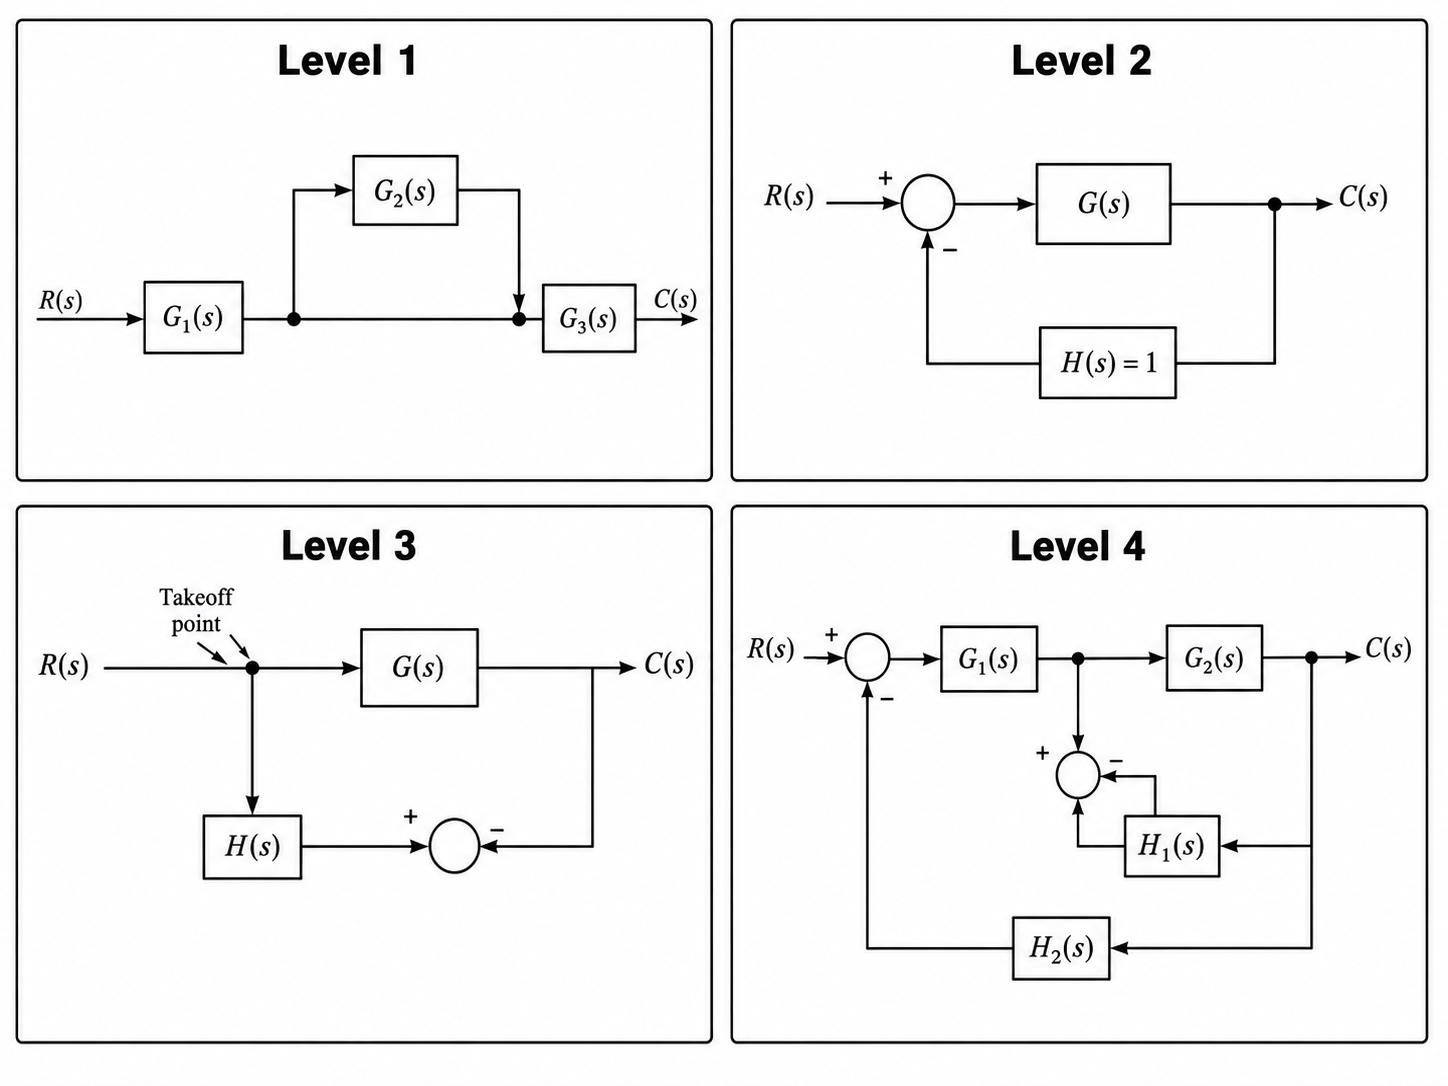
\includegraphics[width=0.8\textwidth]{images/chapter4/figure-08.png}
    \caption{ชุดแผนภาพบล็อกฝึกปฏิบัติ 4 ระดับความยากสำหรับกิจกรรมปฏิบัติการที่ 1}
\end{figure}

\textbf{5. ข้อควรระวังด้านความปลอดภัย:} กิจกรรมนี้เป็นการคำนวณบนกระดาษ ไม่มีความเสี่ยงทางกายภาพ ควรเน้นย้ำให้ผู้เรียนตรวจสอบเครื่องหมายบวกลบและลำดับขั้นตอนอย่างรอบคอบเพื่อป้องกันข้อผิดพลาดทางคณิตศาสตร์

\textbf{6. ขั้นตอนการปฏิบัติ:}
\begin{enumerate}
    \item รับใบงานแผนภาพบล็อกทั้ง 4 ระดับ
    \item วิเคราะห์โครงสร้างและระบุว่าต้องใช้กฎใดบ้างในแต่ละระดับ
    \item ลดรูปทีละขั้นตอน โดยเขียนแสดงทุกขั้นตอนอย่างชัดเจน (ห้ามข้ามขั้นตอน)
    \item เปรียบเทียบคำตอบกับเพื่อนในกลุ่ม (ทำงานเป็นคู่)
    \item ส่งใบงานให้ผู้สอนตรวจสอบ
\end{enumerate}

\textbf{7. ตารางบันทึกผล}

\textbf{ตารางที่ 5} บันทึกผลการลดรูปแผนภาพบล็อกทั้ง 4 ระดับ

\begin{table}[htbp]
    \centering
    \begin{tabular}{l l l l l}
        \hline
        \textbf{ระดับ} & \textbf{กฎที่ใช้ (เรียงลำดับ)} & \textbf{จำนวนขั้นตอน} & \textbf{Transfer Function ที่ได้} & \textbf{ตรวจสอบกับเฉลยแล้ว ($\checkmark$/$\times$)} \\
        \hline
        1 &  &  &  &  \\
        2 &  &  &  &  \\
        3 &  &  &  &  \\
        4 &  &  &  &  \\
        \hline
    \end{tabular}
\end{table}

\textbf{8. การคำนวณและวิเคราะห์ผล:} เปรียบเทียบจำนวนขั้นตอนที่ใช้ในแต่ละระดับ และระบุว่าขั้นตอนใดใช้เวลานานที่สุดหรือเสี่ยงต่อความผิดพลาดมากที่สุด

\textbf{9. การเปรียบเทียบผลกับเฉลย:} ตรวจคำตอบกับเฉลยที่ผู้สอนเตรียมไว้ (ดูหัวข้อ 14 เฉลยแบบฝึกหัด) หากไม่ตรงกัน ให้ย้อนกลับไปตรวจแต่ละขั้นตอน

\textbf{10. คำถามหลังการทดลอง:}
\begin{itemize}
    \item ระดับใดที่ใช้เวลานานที่สุด เพราะเหตุใด
    \item ขั้นตอนการเลื่อนจุดแยกสัญญาณในระดับที่ 3 ทำให้เกิดบล็อกเพิ่มเติมใด และเพราะเหตุใดจึงจำเป็น
    \item ในระดับที่ 4 เหตุใดจึงต้องลดรูปลูปในสุดก่อนลูปนอกสุดเสมอ
\end{itemize}

\textbf{11. เกณฑ์การประเมิน:} ความถูกต้องของ transfer function ที่ได้ในแต่ละระดับ ความครบถ้วนของขั้นตอนที่แสดง และความสามารถในการอธิบายเหตุผลของแต่ละขั้นตอน

\subsubsection{กิจกรรมปฏิบัติการที่ 2: ยืนยันผลด้วยคำสั่ง MATLAB}

\textbf{1. วัตถุประสงค์:} ผู้เรียนสามารถใช้คำสั่ง \texttt{series()}, \texttt{parallel()}, \texttt{feedback()} ใน MATLAB เพื่อยืนยันผลการลดรูปที่คำนวณด้วยมือในกิจกรรมปฏิบัติการที่ 1

\textbf{2. หลักการและทฤษฎีที่เกี่ยวข้อง:} การนิยาม transfer function ด้วย \texttt{tf()} และคำสั่งกลุ่มลดรูปแผนภาพบล็อกใน Control System Toolbox (หัวข้อ 7.8)

\textbf{3. อุปกรณ์ เครื่องมือ และซอฟต์แวร์:} เครื่องคอมพิวเตอร์ที่ติดตั้ง MATLAB พร้อม Control System Toolbox

\textbf{4. แผนภาพหรือวงจร:} ใช้โครงสร้างแผนภาพบล็อกเดียวกันกับกิจกรรมปฏิบัติการที่ 1 ทั้ง 4 ระดับ

\textbf{5. ข้อควรระวังด้านความปลอดภัย:} ไม่มีความเสี่ยงทางกายภาพ ควรตรวจสอบสิทธิ์การใช้งาน MATLAB และ Toolbox ที่จำเป็นก่อนเริ่มกิจกรรม

\textbf{6. ขั้นตอนการปฏิบัติ:}
\begin{enumerate}
    \item เปิด MATLAB และสร้างสคริปต์ใหม่
    \item นิยาม transfer function ของแต่ละบล็อกด้วย \texttt{tf()} ตามใบงาน
    \item ใช้คำสั่ง \texttt{series}, \texttt{parallel}, \texttt{feedback} ตามลำดับโครงสร้างของแต่ละระดับ
    \item แสดงผลลัพธ์ด้วย \texttt{disp()} หรือกราฟการตอบสนองด้วย \texttt{step()}
    \item บันทึกผลลัพธ์และเปรียบเทียบกับคำตอบที่คำนวณด้วยมือ
\end{enumerate}

\textbf{7. ตารางบันทึกผล}

\textbf{ตารางที่ 6} เปรียบเทียบผลจากการคำนวณด้วยมือกับ MATLAB

\begin{table}[htbp]
    \centering
    \small
    \begin{tabularx}{\textwidth}{L{0.10\textwidth} Y Y L{0.18\textwidth}}
        \hline
        \textbf{ระดับ} & \textbf{Transfer Function จากการคำนวณด้วยมือ} & \textbf{Transfer Function จาก MATLAB} & \textbf{ตรงกันหรือไม่ ($\checkmark$/$\times$)} \\
        \hline
        1 &  &  &  \\
        2 &  &  &  \\
        3 &  &  &  \\
        4 &  &  &  \\
        \hline
    \end{tabularx}
\end{table}

\textbf{8. การคำนวณและวิเคราะห์ผล:} ตรวจสอบว่าค่าสัมประสิทธิ์ของพหุนามเศษและส่วนตรงกันหรือไม่ หากไม่ตรงกันให้ระบุจุดที่ผิดพลาด

\textbf{9. การเปรียบเทียบผลกับทฤษฎี:} ผลจาก MATLAB ต้องตรงกับผลการคำนวณด้วยมือทุกระดับ หากไม่ตรงกันให้ตรวจสอบทั้งสองฝั่ง

\textbf{10. คำถามหลังการทดลอง:} คำสั่งใดของ MATLAB ที่ช่วยลดขั้นตอนได้มากที่สุดเมื่อเทียบกับการคำนวณด้วยมือ และเพราะเหตุใด

\textbf{11. เกณฑ์การประเมิน:} ความถูกต้องของสคริปต์ ความตรงกันของผลลัพธ์กับการคำนวณด้วยมือ และการบันทึกเปรียบเทียบอย่างเป็นระบบ

\subsubsection{กิจกรรมปฏิบัติการที่ 3: ยืนยันผลด้วย Simulink}

\textbf{1. วัตถุประสงค์:} ผู้เรียนสามารถสร้างแบบจำลอง Simulink ของระบบเดิม (ไม่ลดรูป) และเปรียบเทียบสัญญาณเอาต์พุตกับแบบจำลองที่ใช้ transfer function รวมที่ลดรูปแล้ว

\textbf{2. หลักการและทฤษฎีที่เกี่ยวข้อง:} การใช้บล็อก Transfer Fcn, Step และ Scope ใน Simulink (หัวข้อ 7.8)

\textbf{3. อุปกรณ์ เครื่องมือ และซอฟต์แวร์:} เครื่องคอมพิวเตอร์ที่ติดตั้ง MATLAB/Simulink

\textbf{4. แผนภาพหรือวงจร:} ใช้ระดับที่ 2 และระดับที่ 4 จากกิจกรรมปฏิบัติการที่ 1 เป็นกรณีศึกษา เนื่องจากมีลูปป้อนกลับที่ชัดเจน

% [รูปที่ 9: ตัวอย่างการจัดวางบล็อกใน Simulink สำหรับยืนยันผลการลดรูป]
% ประเภทภาพ: Experimental Setup
% ตำแหน่งที่แนะนำ: ในกิจกรรมปฏิบัติการที่ 3 หัวข้อที่ 4
% วัตถุประสงค์การเรียนรู้: ให้ผู้เรียนเห็นตัวอย่างการจัดวางบล็อก Simulink ก่อนเริ่มสร้างแบบจำลองจริง
% คำอธิบายภาพ: แสดงบล็อก Step เชื่อมเข้าบล็อก Transfer Fcn สองบล็อกต่ออนุกรมกันในลูปป้อนกลับ ต่อไปยังบล็อก Scope โดยมีจุดแยกสัญญาณย้อนกลับผ่านบล็อกป้อนกลับ Gain เข้าสู่บล็อก Sum ก่อนเข้า Transfer Fcn ตัวแรก จัดวางในลักษณะหน้าต่างแบบจำลอง Simulink
% องค์ประกอบที่ต้องมี: บล็อก Step, Sum, Transfer Fcn (สองบล็อก), Gain (ป้อนกลับ), Scope, เส้นเชื่อมสัญญาณ
% ข้อความหรือป้ายกำกับ: "Step", "Transfer Fcn", "Gain", "Scope", "Sum"
% ภาษาของป้ายกำกับ: อังกฤษ
% สัดส่วนภาพ: 16:9
% Image Generation Prompt: A Simulink model window diagram showing a Step input block connected to a Sum block, then to two Transfer Fcn blocks in series, output going to a Scope block, with a feedback branch through a Gain block returning to the Sum block. Style resembles a simplified Simulink canvas with light gray block outlines and blue signal lines on white background, block labels in clear sans-serif font.
% Alt Text: ภาพตัวอย่างการจัดวางบล็อกในแบบจำลอง Simulink สำหรับยืนยันผลการลดรูปแผนภาพบล็อก

\begin{figure}[htbp]
    \centering
    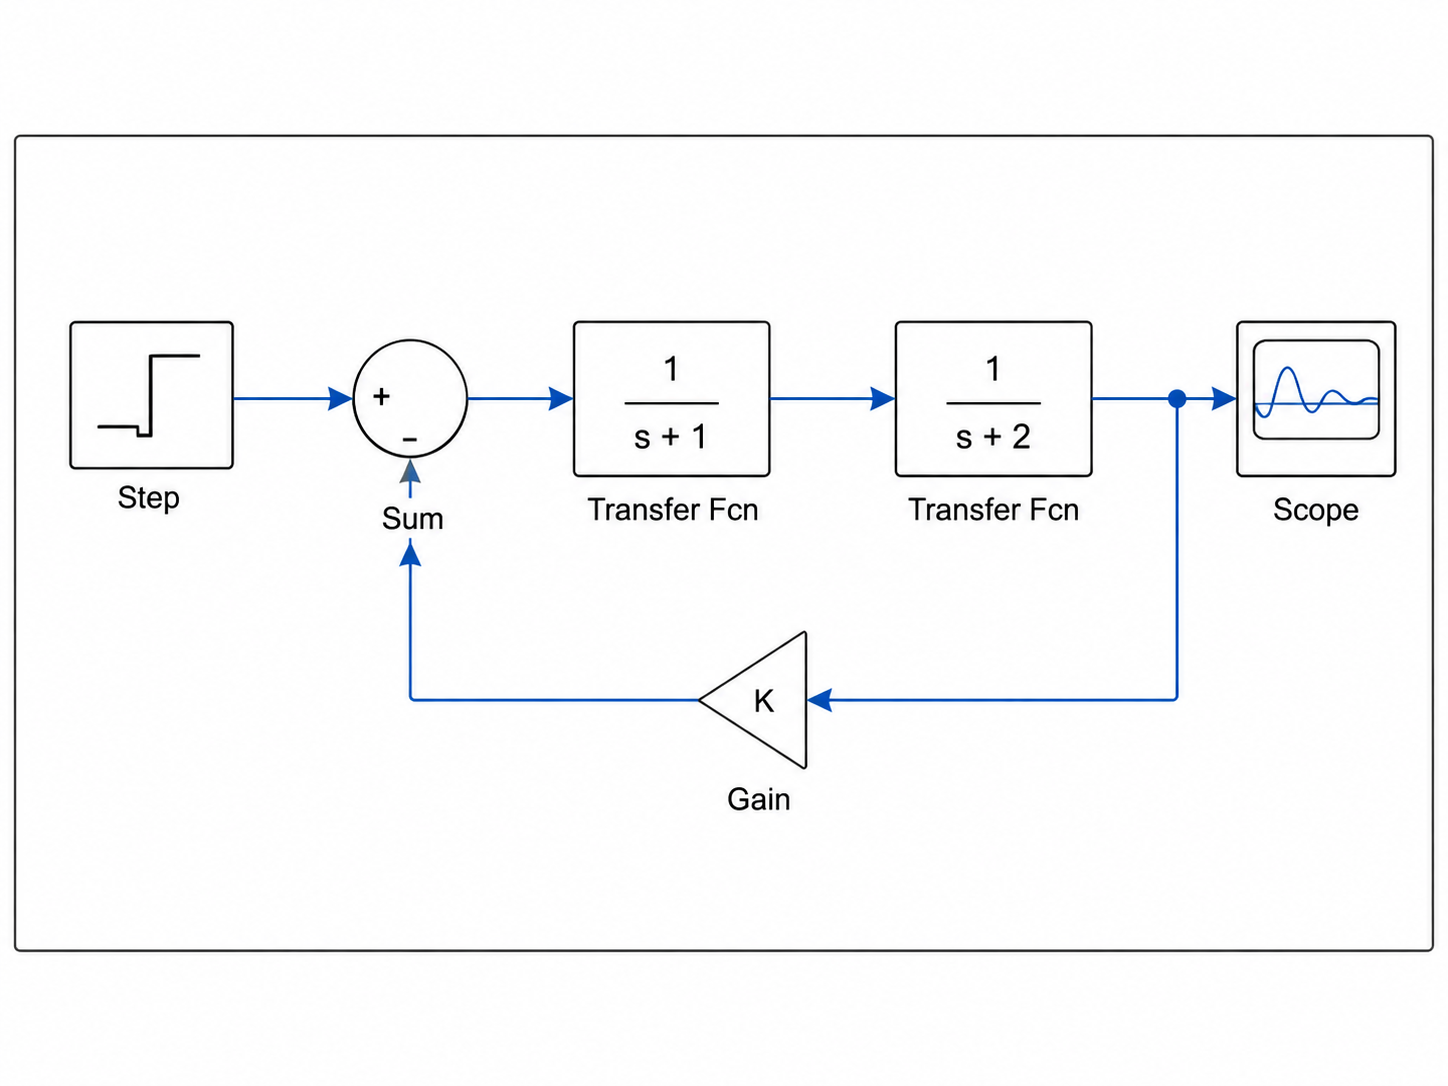
\includegraphics[width=0.8\textwidth]{images/chapter4/figure-09.png}
    \caption{ตัวอย่างการจัดวางบล็อกใน Simulink สำหรับยืนยันผลการลดรูป}
\end{figure}

\textbf{5. ข้อควรระวังด้านความปลอดภัย:} ไม่มีความเสี่ยงทางกายภาพ ควรตั้งค่าเวลาจำลอง (simulation time) และ step size ให้เหมาะสมเพื่อให้ Scope แสดงผลครบช่วงเวลาที่สนใจ

\textbf{6. ขั้นตอนการปฏิบัติ:}
\begin{enumerate}
    \item เปิด Simulink และสร้างแบบจำลองใหม่
    \item วางบล็อก Transfer Fcn ตามโครงสร้างเดิมของระบบ (ไม่ลดรูป) พร้อมบล็อก Sum และ Gain ตามที่จำเป็น
    \item ต่อบล็อก Step เป็นสัญญาณอินพุตและบล็อก Scope ที่เอาต์พุต
    \item รันการจำลองและบันทึกรูปคลื่น
    \item สร้างแบบจำลองที่สองโดยใช้บล็อก Transfer Fcn เพียงตัวเดียวที่มีค่าเท่ากับ transfer function รวมที่ลดรูปแล้ว
    \item เปรียบเทียบรูปคลื่นจากทั้งสอง Scope
\end{enumerate}

\textbf{7. ตารางบันทึกผล}

\textbf{ตารางที่ 7} เปรียบเทียบผลตอบสนองจากแบบจำลอง Simulink ทั้งสองแบบ

\begin{table}[htbp]
    \centering
    \small
    \begin{tabularx}{\textwidth}{L{0.24\textwidth} Y Y L{0.18\textwidth}}
        \hline
        \textbf{กรณี} & \textbf{ค่า Steady-State ที่อ่านได้} & \textbf{เวลาที่เข้าสู่ค่าคงตัวโดยประมาณ (วินาที)} & \textbf{รูปคลื่นซ้อนทับกันหรือไม่ ($\checkmark$/$\times$)} \\
        \hline
        ระดับ 2 (โมเดลไม่ลดรูป) &  &  &  \\
        ระดับ 2 (โมเดลลดรูปแล้ว) &  &  &  \\
        ระดับ 4 (โมเดลไม่ลดรูป) &  &  &  \\
        ระดับ 4 (โมเดลลดรูปแล้ว) &  &  &  \\
        \hline
    \end{tabularx}
\end{table}

\textbf{8. การคำนวณและวิเคราะห์ผล:} หากรูปคลื่นของสองแบบจำลองไม่ซ้อนทับกัน ให้ตรวจสอบพารามิเตอร์บล็อกและเครื่องหมายของสัญญาณป้อนกลับ

\textbf{9. การเปรียบเทียบผลกับทฤษฎี:} ผลจาก Simulink ต้องสอดคล้องกับผลจาก MATLAB ในกิจกรรมปฏิบัติการที่ 2 และผลคำนวณด้วยมือในกิจกรรมปฏิบัติการที่ 1

\textbf{10. คำถามหลังการทดลอง:} เพราะเหตุใดสัญญาณเอาต์พุตของสองแบบจำลองจึงต้องซ้อนทับกันพอดีหากการลดรูปถูกต้อง และหากไม่ซ้อนทับกันควรเริ่มตรวจสอบจากจุดใดก่อน

\textbf{11. เกณฑ์การประเมิน:} ความถูกต้องของการสร้างแบบจำลอง Simulink ความสอดคล้องของผลลัพธ์ระหว่างสองแบบจำลอง และคุณภาพของการวิเคราะห์เมื่อพบความคลาดเคลื่อน

\subsubsection{กิจกรรมปฏิบัติการที่ 4: สร้างตารางช่วยคำนวณ Mason's Gain Formula}

\textbf{1. วัตถุประสงค์:} ผู้เรียนสามารถจัดระบบการคำนวณ Mason's Gain Formula ด้วยตารางช่วยคำนวณที่ครอบคลุม $P_k$, Loop gain, คู่ลูปไม่สัมผัสกัน, $\Delta$ และ $\Delta_k$ เพื่อลดข้อผิดพลาดจากการคำนวณอย่างไม่เป็นระบบ

\textbf{2. หลักการและทฤษฎีที่เกี่ยวข้อง:} Signal Flow Graph และ Mason's Gain Formula (หัวข้อ 7.5–7.6)

\textbf{3. อุปกรณ์ เครื่องมือ และซอฟต์แวร์:} กระดาษ หรือโปรแกรมตารางคำนวณ (เช่น Excel) สำหรับสร้างตาราง

\textbf{4. แผนภาพหรือวงจร:} ใช้ Signal Flow Graph จากตัวอย่างที่ 4 (รูปที่ 7) เป็นกรณีฝึกครั้งแรก จากนั้นผู้สอนอาจเตรียม SFG เพิ่มเติมอีก 1–2 แบบที่มีความซับซ้อนต่างกันสำหรับฝึกเพิ่มเติม

\textbf{5. ข้อควรระวังด้านความปลอดภัย:} ไม่มีความเสี่ยงทางกายภาพ ควรเน้นย้ำการตรวจทานการระบุลูปที่ไม่สัมผัสกันอย่างรอบคอบ เนื่องจากเป็นจุดที่เกิดข้อผิดพลาดบ่อยที่สุด

\textbf{6. ขั้นตอนการปฏิบัติ:}
\begin{enumerate}
    \item รับใบงาน Signal Flow Graph
    \item ระบุเส้นทางหน้าทั้งหมดและกรอกอัตราขยาย $P_k$ ลงในตาราง
    \item ระบุลูปทั้งหมดในกราฟและกรอกอัตราขยายลูปลงในตาราง
    \item ตรวจสอบและกรอกคู่ (หรือกลุ่ม) ของลูปที่ไม่สัมผัสกัน
    \item คำนวณ $\Delta$ จากผลรวมและผลคูณตามสูตร
    \item คำนวณ $\Delta_k$ ของแต่ละเส้นทางหน้า โดยตัดลูปที่สัมผัสกับเส้นทางนั้นออก
    \item แทนค่าในสูตรเมสันเพื่อสรุปผล $C(s)/R(s)$
\end{enumerate}

\textbf{7. ตารางบันทึกผล (Template)}

\textbf{ตารางที่ 8} Template ตารางช่วยคำนวณ Mason's Gain Formula

\begin{table}[htbp]
    \centering
    \begin{tabular}{l l l l l}
        \hline
        \textbf{เส้นทางหน้า/ลูป} & \textbf{โหนดที่ผ่าน} & \textbf{อัตราขยาย ($P_k$ หรือ Loop Gain)} & \textbf{สัมผัสกับลูปใดบ้าง} & \textbf{หมายเหตุ} \\
        \hline
        $P_1$ &  &  &  &  \\
        $P_2$ &  &  &  &  \\
        $L_1$ &  &  &  &  \\
        $L_2$ &  &  &  &  \\
        \hline
    \end{tabular}
\end{table}

\begin{table}[htbp]
    \centering
    \begin{tabular}{l l}
        \hline
        \textbf{คู่ลูปไม่สัมผัสกัน} & \textbf{ผลคูณอัตราขยาย} \\
        \hline
         &  \\
        \hline
    \end{tabular}
\end{table}

\begin{table}[htbp]
    \centering
    \begin{tabular}{l l l}
        \hline
        \textbf{รายการ} & \textbf{สูตร} & \textbf{ค่าที่คำนวณได้} \\
        \hline
        $\Delta$ & $1-\sum L_i+\sum L_iL_j-\cdots$ &  \\
        $\Delta_1$ &  &  \\
        $\Delta_2$ &  &  \\
        $C(s)/R(s)$ & $\dfrac{1}{\Delta}\sum P_k\Delta_k$ &  \\
        \hline
    \end{tabular}
\end{table}

\textbf{8. การคำนวณและวิเคราะห์ผล:} ใช้ตัวอย่างที่ 4 เป็นกรณีอ้างอิงตรวจสอบความถูกต้องของตารางก่อนนำไปใช้กับ SFG ชุดใหม่

\textbf{9. การเปรียบเทียบผลกับเฉลย:} ตรวจคำตอบกับเฉลยที่ผู้สอนเตรียมไว้

\textbf{10. คำถามหลังการทดลอง:} การใช้ตารางช่วยลดข้อผิดพลาดในขั้นตอนใดได้ชัดเจนที่สุดเมื่อเทียบกับการคำนวณอย่างอิสระโดยไม่มีตาราง

\textbf{11. เกณฑ์การประเมิน:} ความครบถ้วนของตาราง ความถูกต้องของ $\Delta$ และ $\Delta_k$ และความถูกต้องของผลลัพธ์สุดท้าย


\subsection{11. สรุปท้ายบท}

Block Diagram เป็นเครื่องมือแสดงความสัมพันธ์เชิงฟังก์ชันของระบบควบคุมด้วยบล็อก จุดรวมสัญญาณ และจุดแยกสัญญาณ ภายใต้สมมติฐานว่าสัญญาณไหลทิศทางเดียวและไม่มีผลโหลดต่อกัน การลดรูปแผนภาพบล็อกอาศัยกฎหลัก 3 กฎ คือ การต่อแบบอนุกรม ($G_1G_2$) การต่อแบบขนาน ($G_1\pm G_2$) และการป้อนกลับ ($G/(1\pm GH)$) ร่วมกับกฎเสริมสำหรับเลื่อนจุดรวมสัญญาณและจุดแยกสัญญาณเมื่อกฎหลักใช้ไม่ได้โดยตรง โดยควรลดรูปลูปในสุดก่อนเสมอเมื่อระบบมีหลายลูปซ้อนกัน

Signal Flow Graph เป็นอีกแนวทางหนึ่งที่แทนความสัมพันธ์เชิงเส้นด้วยโหนดและกิ่ง และใช้ \textbf{Mason's Gain Formula} คำนวณ transfer function รวมได้โดยตรงจากโครงสร้างกราฟ

\[
P = \frac{1}{\Delta}\sum_k P_k\Delta_k, \qquad \Delta = 1-\sum L_i+\sum L_iL_j-\cdots
\]

โดยจุดสำคัญที่สุดคือการระบุ\textbf{ลูปที่ไม่สัมผัสกัน (non-touching loop)} ให้ครบถ้วนทั้งในการคำนวณ $\Delta$ และโคแฟกเตอร์ $\Delta_k$ ของแต่ละเส้นทางหน้า ทั้งสองวิธีให้ผลลัพธ์ transfer function เดียวกันเสมอเมื่อคำนวณถูกต้อง โดย Block Diagram Reduction เหมาะกับระบบที่มีลูปไม่มากและไม่ซ้อนกันซับซ้อน ในขณะที่ Signal Flow Graph กับ Mason's Gain Formula เหมาะกับระบบที่มีหลายลูปซ้อนกันหรือมีหลายเส้นทางหน้า ผลลัพธ์ที่ได้จากทั้งสองวิธีสามารถยืนยันได้ด้วยคำสั่ง MATLAB (\texttt{series}, \texttt{parallel}, \texttt{feedback}) และแบบจำลอง Simulink

\par\noindent\rule{\textwidth}{0.4pt}\par

\subsection{12. คำถามทบทวน}

\begin{enumerate}
    \item Block Diagram ในระบบควบคุมประกอบด้วยองค์ประกอบพื้นฐานใดบ้าง และแต่ละองค์ประกอบทำหน้าที่อย่างไร
    \item เพราะเหตุใดการต่อแบบอนุกรมจึงใช้การคูณ transfer function ในขณะที่การต่อแบบขนานใช้การบวก
    \item จงเขียนสูตร closed-loop transfer function สำหรับระบบป้อนกลับเชิงลบและเชิงบวก พร้อมอธิบายความแตกต่างของเครื่องหมาย
    \item การเลื่อนจุดรวมสัญญาณไปด้านหน้าบล็อกกับด้านหลังบล็อกต้องเพิ่มบล็อกชดเชยต่างกันอย่างไร เพราะเหตุใด
    \item จงอธิบายความแตกต่างระหว่าง Path, Forward Path และ Loop ใน Signal Flow Graph
    \item Non-touching Loop คืออะไร และเหตุใดจึงมีความสำคัญต่อการคำนวณด้วย Mason's Gain Formula
    \item จงเขียน Mason's Gain Formula พร้อมอธิบายความหมายของสัญลักษณ์ $P_k$, $\Delta$ และ $\Delta_k$ ในสูตร
    \item เพราะเหตุใดโคแฟกเตอร์ $\Delta_k$ ของแต่ละเส้นทางหน้าจึงอาจมีค่าไม่เท่ากัน ยกตัวอย่างประกอบ
    \item จงเปรียบเทียบข้อดีและข้อจำกัดของการลดรูปแผนภาพบล็อกกับการใช้ Signal Flow Graph ร่วมกับ Mason's Gain Formula
    \item คำสั่ง MATLAB ใดใช้สำหรับยืนยันผลการต่อแบบอนุกรม ขนาน และป้อนกลับตามลำดับ และแต่ละคำสั่งคำนวณตามสูตรใด
\end{enumerate}

\newpage

\subsection{13. แบบฝึกหัดท้ายบท}

\textit{หมายเหตุ: โจทย์ทั้งหมดในหัวข้อนี้สร้างขึ้นให้สอดคล้องกับเนื้อหาที่อธิบายในบท เฉลยแยกไว้ในหัวข้อ 14 สำหรับผู้สอน}

\subsubsection{ระดับพื้นฐาน}

\textbf{ข้อ 1.} ระบบมีบล็อก $G_1(s)=\dfrac{4}{s+1}$ และ $G_2(s)=\dfrac{2}{s+3}$ ต่อกันแบบอนุกรม จงหา transfer function รวม

\textbf{ข้อ 2.} ระบบมีบล็อก $G_1(s)=\dfrac{5}{s+2}$ และ $G_2(s)=\dfrac{3}{s+4}$ ต่อกันแบบขนานโดยสัญญาณรวมกันด้วยเครื่องหมายบวก จงหา transfer function รวม

\textbf{ข้อ 3.} ระบบป้อนกลับหนึ่งหน่วยเชิงลบมี $G(s)=\dfrac{6}{s+1}$ จงหา closed-loop transfer function

\textbf{ข้อ 4.} จงระบุว่า Signal Flow Graph ที่มีโหนด $R \to 1 \to 2 \to C$ (ไม่มีลูปย้อนกลับ) มีเส้นทางหน้ากี่เส้นทาง และมีลูปหรือไม่

\textbf{ข้อ 5.} จงอธิบายความแตกต่างระหว่างจุดรวมสัญญาณและจุดแยกสัญญาณ พร้อมยกตัวอย่างระบบที่พบทั้งสององค์ประกอบ

\subsubsection{ระดับวิเคราะห์}

\textbf{ข้อ 6.} ระบบมีเส้นทางไปข้างหน้า $G(s)=\dfrac{8}{s(s+3)}$ และป้อนกลับเชิงลบผ่าน $H(s)=0.5$ จงหา closed-loop transfer function และระบุตำแหน่งขั้ว (pole)

\textbf{ข้อ 7.} แผนภาพบล็อกมี $G_1(s)=\dfrac{2}{s+1}$ ต่ออนุกรมกับ $G_2(s)=\dfrac{3}{s+2}$ แล้วผลลัพธ์รวมมีลูปป้อนกลับเชิงลบผ่าน $H(s)=1$ จงลดรูปเป็น transfer function เดียว

\textbf{ข้อ 8.} Signal Flow Graph มีเส้นทางหน้าเดียว $P_1 = G_1G_2G_3$ และลูปสองลูปที่\textbf{สัมผัสกัน} (มีโหนดร่วม) คือ $L_1$ และ $L_2$ จงเขียนสูตรคำนวณ $\Delta$ ของกราฟนี้ พร้อมอธิบายว่าเหตุใดจึงไม่มีพจน์ $L_1L_2$ ในสูตร

\textbf{ข้อ 9.} จงเปรียบเทียบจำนวนขั้นตอนที่ต้องใช้ในการหา transfer function ของระบบที่มี 3 ลูปป้อนกลับซ้อนกัน ระหว่างวิธีลดรูปแผนภาพบล็อกกับวิธี Mason's Gain Formula

\textbf{ข้อ 10.} ระบบมีจุดแยกสัญญาณอยู่ก่อนบล็อก $G(s)=\dfrac{1}{s+5}$ และจำเป็นต้องเลื่อนจุดแยกสัญญาณไปด้านหลังบล็อกเพื่อรวมกับบล็อกอื่น จงระบุบล็อกชดเชยที่ต้องเพิ่มในเส้นสัญญาณที่แยกออกไป

\subsubsection{ระดับประยุกต์ใช้}

\textbf{ข้อ 11.} ระบบควบคุมความเร็วมอเตอร์มีตัวควบคุม $G_c(s)=\dfrac{K}{s}$ (โดย $K=4$) ต่ออนุกรมกับมอเตอร์ $G_m(s)=\dfrac{2}{s+5}$ และมีเซนเซอร์ป้อนกลับ $H(s)=0.1$ จงหา closed-loop transfer function ของระบบทั้งหมด และยืนยันผลด้วยคำสั่ง MATLAB \texttt{series} และ \texttt{feedback}

\textbf{ข้อ 12.} ระบบควบคุมท่าทางมีลูปในควบคุมอัตราการหมุน (inner loop) และลูปนอกควบคุมมุม (outer loop) ซ้อนกัน จงอธิบายว่าเหตุใดวิศวกรจึงมักเลือกใช้ Signal Flow Graph แทนการลดรูปแผนภาพบล็อกทีละขั้นตอนสำหรับระบบลักษณะนี้ พร้อมยกเหตุผลสนับสนุนอย่างน้อย 2 ข้อ

\textbf{ข้อ 13.} จงสร้าง Signal Flow Graph ของระบบที่มีสองเส้นทางหน้าและสองลูปที่\textbf{ไม่สัมผัสกัน} ขึ้นเองหนึ่งชุด (กำหนดอัตราขยายเป็นสัญลักษณ์ได้) แล้วคำนวณ transfer function รวมด้วย Mason's Gain Formula พร้อมแสดงตารางช่วยคำนวณตามรูปแบบในหัวข้อกิจกรรมปฏิบัติการที่ 4

\par\noindent\rule{\textwidth}{0.4pt}\par

\newpage

\subsection{14. เฉลยแบบฝึกหัด (สำหรับผู้สอน)}

\textit{หมายเหตุ: หัวข้อนี้จัดทำสำหรับผู้สอนใช้ตรวจสอบคำตอบ หากต้องการจัดทำเอกสารสำหรับนักศึกษาโดยไม่เปิดเผยคำตอบ ให้แยกหัวข้อนี้ออกเป็นไฟล์ต่างหาก}

\subsubsection{เฉลยระดับพื้นฐาน}

\textbf{ข้อ 1.} ใช้กฎการต่อแบบอนุกรม:
\[
G_{eq}(s)=G_1(s)G_2(s)=\dfrac{4}{s+1}\cdot\dfrac{2}{s+3}
=\dfrac{8}{(s+1)(s+3)}=\dfrac{8}{s^2+4s+3}
\]
คำตอบ: $\dfrac{8}{s^2+4s+3}$ ข้อผิดพลาดที่พบบ่อย: นักศึกษามักบวกแทนที่จะคูณ

\textbf{ข้อ 2.} ใช้กฎการต่อแบบขนาน: $G_{eq}(s)=\dfrac{5}{s+2}+\dfrac{3}{s+4}=\dfrac{5(s+4)+3(s+2)}{(s+2)(s+4)}=\dfrac{8s+26}{s^2+6s+8}$ — คำตอบ: $\dfrac{8s+26}{s^2+6s+8}$

\textbf{ข้อ 3.} ใช้สูตรป้อนกลับเชิงลบ: $\dfrac{C(s)}{R(s)}=\dfrac{G(s)}{1+G(s)}=\dfrac{6/(s+1)}{1+6/(s+1)}=\dfrac{6}{s+7}$ — คำตอบ: $\dfrac{6}{s+7}$ การแปลความหมาย: ขั้วเลื่อนจาก $s=-1$ (open-loop) ไปที่ $s=-7$ (closed-loop) แสดงว่าระบบตอบสนองเร็วขึ้นเมื่อปิดลูป

\textbf{ข้อ 4.} มีเส้นทางหน้าเพียง 1 เส้นทาง ($R\to1\to2\to C$) และ\textbf{ไม่มีลูป}เนื่องจากไม่มีกิ่งใดย้อนกลับไปยังโหนดที่ผ่านมาแล้ว

\textbf{ข้อ 5.} จุดรวมสัญญาณรวมสัญญาณตั้งแต่สองสัญญาณขึ้นไปด้วยการบวกหรือลบ (เช่น จุดเปรียบเทียบค่าอ้างอิงกับสัญญาณป้อนกลับ) ส่วนจุดแยกสัญญาณแยกสัญญาณเดียวส่งไปหลายเส้นทางโดยไม่เปลี่ยนค่า (เช่น จุดที่ส่งสัญญาณเอาต์พุตไปทั้งโหลดและกลับไปยังเซนเซอร์ป้อนกลับพร้อมกัน)

\subsubsection{เฉลยระดับวิเคราะห์}

\textbf{ข้อ 6.} $\dfrac{C(s)}{R(s)}=\dfrac{G(s)}{1+G(s)H(s)}=\dfrac{8/[s(s+3)]}{1+0.5\cdot8/[s(s+3)]}=\dfrac{8}{s(s+3)+4}=\dfrac{8}{s^2+3s+4}$ ขั้วอยู่ที่รากของ $s^2+3s+4=0$ คือ $s=\dfrac{-3\pm\sqrt{9-16}}{2}=-1.5\pm j1.32$ (ขั้วเชิงซ้อนคู่ควบ)

\textbf{ข้อ 7.} ลดรูปอนุกรมก่อน: $G_1G_2=\dfrac{2}{s+1}\cdot\dfrac{3}{s+2}=\dfrac{6}{(s+1)(s+2)}$ จากนั้นปิดลูปป้อนกลับหนึ่งหน่วยเชิงลบ: $\dfrac{6/[(s+1)(s+2)]}{1+6/[(s+1)(s+2)]}=\dfrac{6}{(s+1)(s+2)+6}=\dfrac{6}{s^2+3s+8}$

\textbf{ข้อ 8.} $\Delta = 1-(L_1+L_2)$ เนื่องจาก $L_1$ และ $L_2$ สัมผัสกัน (มีโหนดร่วม) จึงไม่มีคู่ลูปไม่สัมผัสกันให้พิจารณา พจน์ $L_1L_2$ (ผลคูณของคู่ลูปไม่สัมผัสกัน) จึงไม่ปรากฏในสูตร

\textbf{ข้อ 9.} วิธีลดรูปแผนภาพบล็อกต้องเลื่อนจุดรวม/จุดแยกสัญญาณและลดรูปทีละลูปจากในสุดไปนอกสุด ใช้หลายขั้นตอนและเสี่ยงต่อความผิดพลาดสะสม ส่วนวิธี Mason's Gain Formula คำนวณ $\Delta$ และ $\Delta_k$ จากโครงสร้างกราฟได้โดยตรงในขั้นตอนเดียว จึงมักใช้ขั้นตอนน้อยกว่าเมื่อระบบมีลูปซ้อนกันหลายชั้น แต่ต้องระบุลูปไม่สัมผัสกันให้ครบถ้วน

\textbf{ข้อ 10.} ต้องเพิ่มบล็อก $1/G(s) = (s+5)$ เข้าที่เส้นสัญญาณที่แยกออกไป เพื่อให้ค่าสัญญาณที่จุดแยกเดิมไม่เปลี่ยนแปลงหลังเลื่อนตำแหน่ง

\subsubsection{เฉลยระดับประยุกต์ใช้}

\textbf{ข้อ 11.} ลดรูปอนุกรมก่อน: $G_c(s)G_m(s)=\dfrac{4}{s}\cdot\dfrac{2}{s+5}=\dfrac{8}{s(s+5)}=\dfrac{8}{s^2+5s}$ จากนั้นปิดลูปป้อนกลับ: $\dfrac{C(s)}{R(s)}=\dfrac{8/(s^2+5s)}{1+0.1\cdot8/(s^2+5s)}=\dfrac{8}{s^2+5s+0.8}$ ตรวจสอบด้วย MATLAB: \texttt{G = series(tf([4],[1 0]), tf([2],[1 5])); Gcl = feedback(G, 0.1);} ผลลัพธ์ที่ได้ต้องมีสัมประสิทธิ์ตรงกับที่คำนวณด้วยมือ

\textbf{ข้อ 12.} เหตุผลสนับสนุน ได้แก่ (1) ระบบมีลูปซ้อนกันตั้งแต่สองชั้นขึ้นไป การลดรูปแผนภาพบล็อกทีละขั้นตอนต้องเลื่อนจุดรวม/จุดแยกสัญญาณหลายครั้งและเสี่ยงต่อข้อผิดพลาดสะสม ในขณะที่ Mason's Gain Formula คำนวณจากโครงสร้างกราฟได้โดยตรง (2) หากมีการปรับพารามิเตอร์ของลูปใดลูปหนึ่งภายหลัง (เช่น ปรับอัตราขยายตัวควบคุม) การคำนวณใหม่ด้วย SFG ทำได้รวดเร็วกว่าเพราะไม่ต้องไล่ลดรูปใหม่ทั้งหมด

\textbf{ข้อ 13.} คำตอบขึ้นอยู่กับ SFG ที่นักศึกษาสร้างขึ้นเอง ผู้สอนควรตรวจสอบว่า (1) มีเส้นทางหน้าสองเส้นทางจริงและไม่ผ่านโหนดซ้ำ (2) สองลูปที่ระบุไม่มีโหนดร่วมกันจริง (3) การคำนวณ $\Delta$ และ $\Delta_k$ เป็นไปตามสูตรและสอดคล้องกับตัวอย่างที่ 4 ในเนื้อหา


\subsection{15. ข้อเสนอแนะสำหรับผู้สอน}

\begin{itemize}
    \item \textbf{ลำดับการสอน:} แนะนำให้สอนกฎการลดรูปแผนภาพบล็อก (หัวข้อ 7.3) ให้แน่นก่อนจึงเข้าสู่ Signal Flow Graph และ Mason's Gain Formula เนื่องจากผู้เรียนจะเข้าใจที่มาของสูตรป้อนกลับได้ง่ายกว่าเมื่อผ่านการฝึกลดรูปด้วยกฎพีชคณิตมาก่อน
    \item \textbf{สำหรับนักศึกษาสาย ม.6:} ให้สอนการลดรูปแผนภาพบล็อกทีละขั้นตอนอย่างละเอียดก่อน โดยเน้นตัวอย่างที่ 1–3 ให้คล่องก่อนขยับไปสู่ Signal Flow Graph เพื่อไม่ให้ผู้เรียนสับสนระหว่างสองแนวคิดพร้อมกัน
    \item \textbf{สำหรับนักศึกษาสาย ปวช.:} แนะนำให้ใช้ Template ตารางคำนวณ Mason's Gain Formula (ตารางที่ 8 ในกิจกรรมปฏิบัติการที่ 4) ตั้งแต่เริ่มฝึก เพื่อลดข้อผิดพลาดจากการคำนวณอย่างไม่เป็นระบบ
    \item \textbf{จุดที่ผู้เรียนมักมีปัญหา:} การลืมบวกกลับด้วยผลคูณของคู่ลูปไม่สัมผัสกันเมื่อคำนวณ $\Delta$ และการใช้ $\Delta$ เดียวกับทุกเส้นทางหน้าโดยไม่แยกคำนวณ $\Delta_k$ ผู้สอนควรเน้นย้ำจุดนี้ด้วยตัวอย่างที่ 4 ซ้ำหลายครั้งจนผู้เรียนคล่อง
    \item \textbf{วิธีเลือกตัวอย่างเพิ่มเติม:} หากต้องการโจทย์เพิ่มเติม ควรเริ่มจากระบบที่มีเพียงหนึ่งลูปก่อน แล้วค่อยเพิ่มจำนวนลูปและเส้นทางหน้าทีละน้อย เพื่อให้ผู้เรียนเห็นพัฒนาการของความซับซ้อนอย่างเป็นลำดับ
    \item \textbf{แนวทางประเมินระหว่างเรียน:} ใช้คำถามกระตุ้นความคิดสั้น ๆ ระหว่างบรรยาย เช่น ให้ผู้เรียนระบุว่าโครงสร้างที่แสดงบนกระดานเป็นการต่อแบบใด ก่อนเฉลย เพื่อตรวจสอบความเข้าใจแบบทันที (formative assessment) และปรับจังหวะการสอนตามความเข้าใจของชั้นเรียน
\end{itemize}


\subsection{16. สื่อและแหล่งเรียนรู้เพิ่มเติม}

\begin{itemize}
    \item \textbf{NPTEL:} วิดีโอหัวข้อ Block Diagram Reduction และ Signal Flow Graph ในรายวิชา Control Systems คำค้นแนะนำ: "Block Diagram Reduction Control Systems", "Signal Flow Graph Control Systems" เหมาะสำหรับทบทวนหลังบรรยายหัวข้อ 7.3 และ 7.5
    \item \textbf{คำค้นวิดีโอ "Mason Gain Formula":} ใช้ค้นหาวิดีโอประกอบการอธิบายขั้นตอนการคำนวณ Mason's Gain Formula เหมาะสำหรับทบทวนก่อนทำกิจกรรมปฏิบัติการที่ 4
    \item \textbf{MathWorks Documentation:} เอกสารและตัวอย่าง (MATLAB examples) เกี่ยวกับคำสั่ง \texttt{feedback}, \texttt{series}, \texttt{parallel} ใน Control System Toolbox เหมาะสำหรับใช้ประกอบกิจกรรมปฏิบัติการที่ 2 โดยให้ผู้เรียนค้นหาจากเว็บไซต์ MathWorks โดยตรงเพื่อดูตัวอย่างการใช้งานฉบับล่าสุด
\end{itemize}

\textit{หมายเหตุ: รายการข้างต้นเป็นแนวทางค้นหาตามที่ผู้ใช้ระบุ ไม่มีการแต่งชื่อคลิป ลิงก์ ผู้บรรยาย หรือปีเผยแพร่ขึ้นเอง ผู้สอนควรตรวจสอบและเลือกคลิปที่เหมาะสมกับเนื้อหาก่อนนำไปใช้จริง}

\par\noindent\rule{\textwidth}{0.4pt}\par

\subsection{17. เอกสารอ้างอิง}

\textit{หมายเหตุ: รายการต่อไปนี้เป็นแหล่งอ้างอิงมาตรฐานในสาขาระบบควบคุมที่ตรงกับเนื้อหาของบทนี้ ผู้สอนควรตรวจสอบรายละเอียดฉบับพิมพ์ (edition, ปีพิมพ์, สำนักพิมพ์) ให้ตรงกับฉบับที่ใช้อ้างอิงจริงก่อนเผยแพร่}

\begin{enumerate}
    \item Ogata, K. (2010). \textit{Modern Control Engineering} (5th ed.). Prentice Hall. — บทที่ว่าด้วย Block Diagrams และ Signal Flow Graphs
    \item Nise, N. S. (2015). \textit{Control Systems Engineering} (7th ed.). Wiley. — บทที่ว่าด้วย Reduction of Multiple Subsystems และ Mason's Rule
    \item Dorf, R. C., \& Bishop, R. H. (2017). \textit{Modern Control Systems} (13th ed.). Pearson. — บทที่ว่าด้วย The Control System
    \item MathWorks. \textit{Control System Toolbox Documentation: series, parallel, feedback}. เว็บไซต์ทางการของ MathWorks (ตรวจสอบ URL ฉบับล่าสุดก่อนอ้างอิงในเอกสารเผยแพร่)
    \item NPTEL (National Programme on Technology Enhanced Learning). วิดีโอบรรยายหัวข้อ Block Diagram Reduction และ Signal Flow Graph ในรายวิชา Control Systems (ตรวจสอบชื่อผู้บรรยายและลิงก์ฉบับล่าสุดก่อนอ้างอิง)
\end{enumerate}
